\documentclass{article}
\usepackage{iclr2027_conference,times}
\input{math_commands.tex}
\usepackage{hyperref}
\usepackage{url}
\usepackage{amsthm}
\usepackage{booktabs}
\usepackage{placeins}
\usepackage{graphicx}
\usepackage{microtype}
\pdfminorversion=7

% Allow figures and tables to share text pages instead of forming a late float queue.
\renewcommand{\topfraction}{0.95}
\renewcommand{\bottomfraction}{0.95}
\renewcommand{\textfraction}{0.05}
\renewcommand{\floatpagefraction}{0.85}
\setcounter{topnumber}{3}
\setcounter{bottomnumber}{3}
\setcounter{totalnumber}{5}
\setlength{\textfloatsep}{9pt plus 1pt minus 2pt}
\setlength{\floatsep}{7pt plus 1pt minus 2pt}
\setlength{\intextsep}{6pt plus 1pt minus 2pt}
\setlength{\abovecaptionskip}{5pt}

\newtheorem{proposition}{Proposition}[section]
\newtheorem{lemma}[proposition]{Lemma}
\newtheorem{theorem}[proposition]{Theorem}

\title{AdaSolver: Efficient Neural Operator Inference via Test-Time Adaptive Sampling}
\author{Anonymous Authors}

\begin{document}
\maketitle

\begin{abstract}
Neural operators provide efficient surrogates for partial differential equations (PDEs), yet their inference performance is typically tied to uniform spatial discretizations or sampling schemes. Many PDE solutions exhibit localized structures that require dense sampling for accurate prediction, while smooth regions can be represented with substantially fewer points. Naively changing the sampling density, however, shifts the empirical input measure and can introduce sampling-dependent bias into the learned neural operator. We introduce \textbf{AdaSolver}, a measure-aware framework for adaptive spatial computation at test time. We characterize sampling-induced bias and its propagation through physics-attention, and derive a sampling-density-consistent Transolver using self-normalized importance weighting. The resulting measure-consistent formulation  preserves consistency with the reference measure, enabling adaptive test-time sampling across different physical systems and geometric designs. Building on this formulation, we explore three refinement strategies based on physics-informed priors, coarse-prediction guidance, and cache-aware learned refinement. Across five standard PDE benchmarks and three industrial aerodynamic tasks, AdaSolver improves prediction accuracy under matched sampling budgets and accelerates surrogate-based airfoil and wing optimization. These results establish adaptive spatial sampling as a principled axis of test-time scaling for neural operators.
\end{abstract}

\section{Introduction}

Neural operators learn maps between function spaces and can amortize expensive numerical simulation across many physical configurations \citep{li2021fno,li2023gino,wu2024transolver}. Recently, transformer-based neural operators have improved the scalability and accuracy of operator learning across diverse PDEs and million-point geometries. They make such large-scale computation possible by compressing irregular meshes into latent tokens, distributing the computation, or decoupling global state estimation from pointwise decoding \citep{alkin2024upt,luo2025transolverpp,zhou2026transolver3}. In engineering applications, however, evaluation efficiency is as important as scalability. Yet how neural operators can flexibly allocate computation at inference remains largely unexplored.

Neural-operator training data are typically generated by numerical solvers on meshes that are uniform or designed for numerical convergence. Learned models are consequently evaluated under the same sampling distribution, which may ignore the strongly localized structure of many PDE solutions. Shocks, boundary layers, contact interfaces, and stress concentrations often occur in localized regions and require finer resolution, whereas smooth regions can be represented with fewer samples. This creates a dilemma: preserving the training distribution wastes samples in smooth regions, while reallocating them to critical regions changes the sampling measure. Can a neural operator reallocate a given sampling budget without changing the operator it represents?


Existing efforts address neighboring capabilities. First, resolution
generalization studies how neural operators extrapolate across grid sizes,
point counts, or compatible discretizations while preserving the underlying
sampling distribution \citep{li2021fno,li2023gino,liu2023nuno,alkin2024upt,
zhou2026transolver3,gao2025discretization}. These methods make resolution
changes feasible, but do not by themselves provide a mechanism for spatially reallocating samples according to local physical or solution structures. Second, adaptive sampling and refinement
methods predict where a numerical mesh or point set should be refined, often
as part of a solver pipeline or through a separately trained refinement model
\citep{huang2021meshgeneration,obiols2023adarnet,rowbottom2024gadaptivity}.
They address spatial allocation, but do not specify how a frozen neural
operator should preserve its target integral when that allocation changes the
sampling measure. Third, test-time compute scaling increases inference effort
through adaptive reasoning or iterative physical prediction
\citep{snell2024scalingllmtesttime,lippe2023pderefiner,jenkins2026atca,
serrano2026splitting}. These works establish the value of allocating additional
computation at inference, but leave open the spatial counterpart: reallocating
input samples for operator evaluation while retaining the same learned map.

We introduce AdaSolver to address this gap. We view spatial sampling density as a controllable inference resource for allocating computation at test time. From a continuous-operator perspective, we characterize how shifts in sampling density introduce sampling bias into Transolver. We develop a sampling-density-consistent Transolver that corrects this bias through self-normalized importance weighting. This measure correction enables adaptive test-time sampling driven by geometry or physics priors, a low-cost coarse prediction, or a cache-aware learned refinement policy that reuses intermediate features. Figure~\ref{fig:adasolver_overview} illustrates the AdaSolver framework and its alternative test-time sampling strategies.
\begin{figure}[h!]
    \centering
    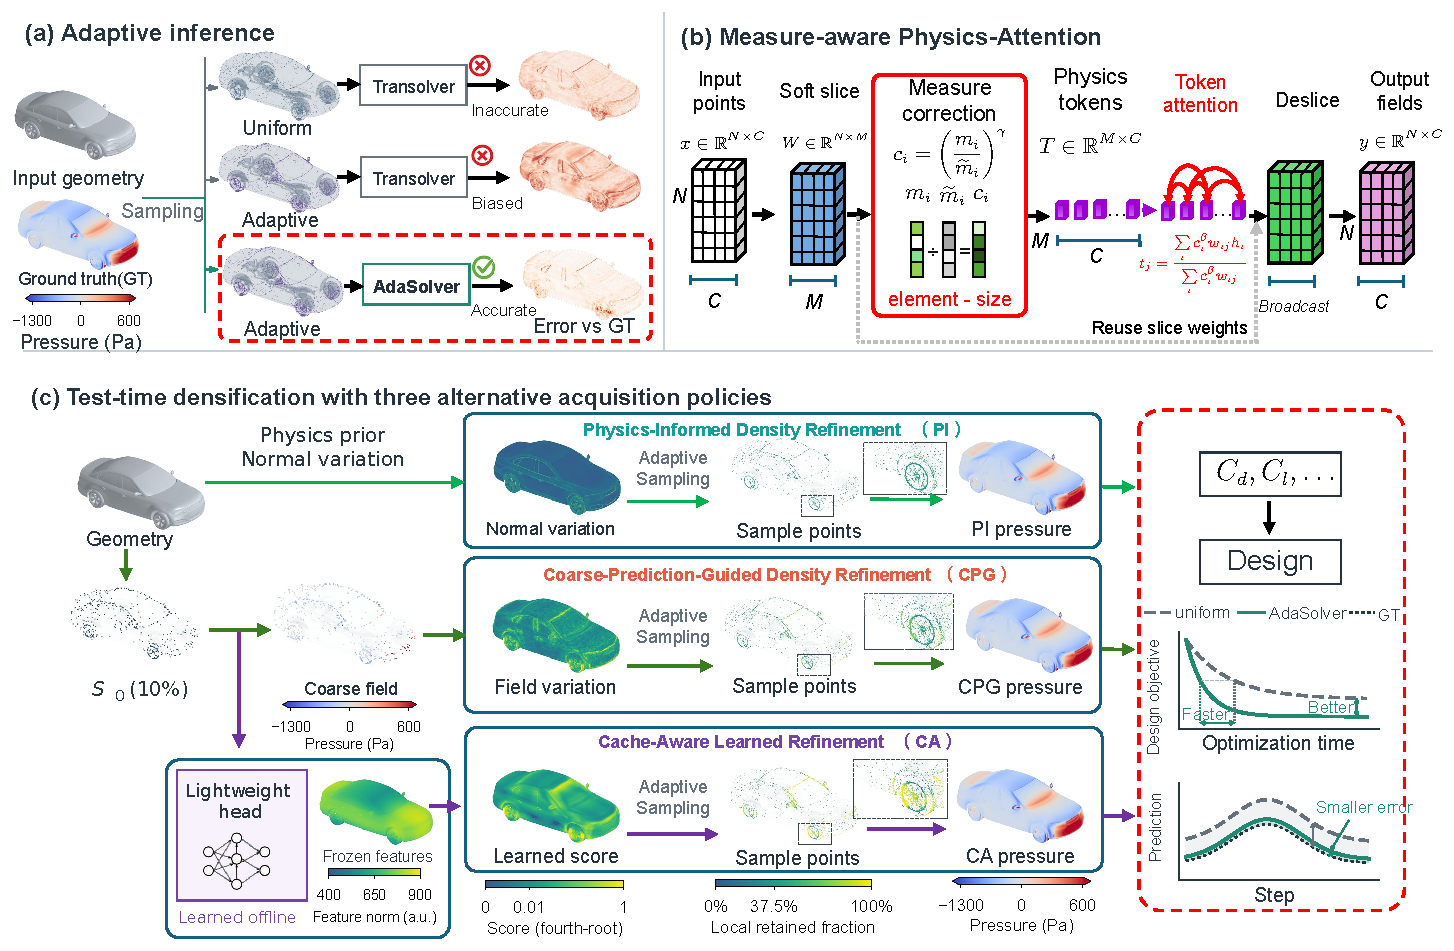
\includegraphics[width=\linewidth]{figures/fig1_overview.pdf}
    \caption{\textbf{AdaSolver overview.}
    (a) Adaptive inference with measure correction.
    (b) Corrected aggregation, token attention, and deslicing.
    (c) Geometry priors, coarse predictions, and a lightweight head on frozen
    features provide alternative refinement signals. The frozen operator evaluates
    the selected points and supplies aerodynamic quantities for design. The
    rightmost curves illustrate the design objectives schematically.}
    \label{fig:adasolver_overview}
\end{figure}


We summarize our contributions as follows: (i) to our knowledge, we provide the first systematic exploration of adaptive spatial sampling as a new axis of test-time scaling for neural operators, revealing sampling-measure shift as a fundamental challenge when reallocating spatial computation at inference; (ii) we introduce AdaSolver, which enables measure-consistent test-time sampling and supports diverse scaling strategies based on physics and geometry priors, coarse predictions, and learned refinement signals; and (iii) we demonstrate consistent improvements in the accuracy--compute trade-off across five standard PDE benchmarks and three industrial aerodynamic tasks, and further show that AdaSolver accelerates surrogate-based airfoil and wing optimization while achieving comparable or improved CFD-validated aerodynamic performance.

\section{Related Work}

\paragraph{Neural operators on irregular geometries.}
Fourier neural operators learn resolution-transferable spectral mappings on
regular grids, while Geo-FNO extends them to general geometries through learned
coordinate deformations \citep{li2021fno,li2023geofno}. GINO couples integral
operators with a latent regular grid, and NUNO partitions non-uniform
observations to reduce interpolation and computational costs
\citep{li2023gino,liu2023nuno}. Transformer-based operators instead compress
large point sets into latent representations before global interaction, as in
GNOT, UPT, and Transolver \citep{hao2023gnot,alkin2024upt,wu2024transolver}.
Transolver++ and Transolver-3 further scale this design to million-scale and
industrial-scale geometries \citep{luo2025transolverpp,zhou2026transolver3}.
These methods establish strong compatibility with irregular inputs and changing
point counts. Our focus is complementary: we actively change the \emph{local}
sampling density at inference and ask whether the frozen model still represents
the same continuous operator.

\paragraph{Discretization-consistent operator learning.}
Extending finite neural architectures to function spaces requires discrete
reductions to converge to fixed continuous integrals as the discretization
changes \citep{berner2026functionspaces}. Monte Carlo convolution corrects
non-uniform point-cloud sampling with inverse-density weights, while QuadConv
evaluates continuous kernels using quadrature on irregular PDE data
\citep{hermosilla2018montecarlo,doherty2024quadconv}. Related formulations
construct discretization-invariant maps between neural fields and
quadrature-aware normalization statistics \citep{wang2022din,kim2026quadnorm}.
Nevertheless, resolution-independent parameters alone do not prevent errors
under a mismatch between training and evaluation discretizations
\citep{gao2025discretization}. We adopt the same function-space principle for
latent point aggregation, but use it to support a deliberate inference-time
change of sampling density rather than only passive resolution transfer.

\paragraph{Adaptive meshes and test-time refinement.}
Adaptive discretization concentrates resolution where numerical error is
expected to be large. Learned approaches predict mesh density, refinement, or
node relocation for numerical solvers
\citep{huang2021meshgeneration,obiols2023adarnet,rowbottom2024gadaptivity},
while MeshGraphNets integrates learned dynamics with mesh-based simulation
\citep{pfaff2021meshgraphnets}. Test-time computation has also been increased
through iterative denoising in PDE-Refiner, adaptive allocation or tokenization,
and neural-operator composition
\citep{lippe2023pderefiner,jenkins2026atca,
wang2026adaptivetokenization,serrano2026splitting}. These directions determine
where or how additional inference computation should be used. AdaSolver
addresses the complementary operator-level requirement: changing the spatial
sampling density of a frozen point-based neural operator while keeping its
reference continuous measure fixed.

\vspace{-2em}
\section{Method}
\paragraph{Transformer neural operators.}
Transformer neural operators use attention to discretize nonlocal integral operators over a physical domain~$\Omega$. Let $\rho$ denote the prescribed sampling measure on $\Omega$, which encodes whether points lie on a surface or in a volume as well as the density induced by a meshing or numerical refinement policy. Given $N$ discretization points $\{\xi_n\}_{n=1}^{N}$ sampled from $\rho$, an unweighted average over the points approximates an integral with respect to $\rho$.

OFormer~\citep{li2023oformer} performs this approximation directly in the point space. Omitting attention-head indices, its Galerkin attention can be written as
\begin{equation}
    y_c(\xi_i)
    = \sum_{\ell=1}^{d} q_\ell(\xi_i)
      \left(\frac{1}{N}\sum_{n=1}^{N}
      \widehat{k}_\ell(\xi_n)\widehat{v}_c(\xi_n)\right)
    \xrightarrow[N\to\infty]{}
    \sum_{\ell=1}^{d} q_\ell(\xi_i)
      \int_{\Omega}\widehat{k}_\ell(\xi)\widehat{v}_c(\xi)
      \mathrm{d}\rho(\xi),
    \label{eq:oformer_galerkin}
\end{equation}
where $d$ is the attention width, $q_\ell$ and $k_\ell$ are learned basis functions, $v_c$ is a value channel, and the hats denote the column-wise normalization used by OFormer. Thus, $\widehat{K}^{\top}\widehat{V}/N$ estimates basis inner products by quadrature, while $Q$ reconstructs the output at each query point.

Transolver~\citep{wu2024transolver} replaces point-to-point attention with Physics-Attention, which first groups point features into a small number of learned physical states. Let $h_n=h(\xi_n)\in\mathbb{R}^{C}$ denote the feature at point $\xi_n$. A point-wise projection $p:\mathbb{R}^{C}\rightarrow\mathbb{R}^{M}$ produces the slice weights
\begin{equation}
    a_{nj}
    = \left[\operatorname{softmax}\!\left(\frac{p(h_n)}{\tau_0}\right)\right]_j,
    \qquad
    \sum_{j=1}^{M}a_{nj}=1,
    \label{eq:transolver_weights}
\end{equation}
where $M$ is the number of slices and $\tau_0$ is a temperature. The weights are computed from features rather than spatial coordinates, so points that share a physical state can be assigned to the same slice even when they are far apart in $\Omega$. For each slice, Physics-Attention forms a normalized physical state by weighted aggregation:
\begin{equation}
    s_j^{(N)}
    = \frac{\sum_{n=1}^{N}a_{nj}h_n}
           {\sum_{n=1}^{N}a_{nj}}
    \xrightarrow[N\to\infty]{}
    s_j^{\rho}
    = \frac{\int_{\Omega}a_j(\xi)h(\xi)\,\mathrm{d}\rho(\xi)}
           {\int_{\Omega}a_j(\xi)\,\mathrm{d}\rho(\xi)}.
    \label{eq:transolver_slice}
\end{equation}
Thus, the physical state is a conditional average under the sampling measure $\rho$, rather than a value associated with a fixed spatial cell. This normalization is also the point at which the empirical sampling distribution enters the point-to-state aggregation.

Let $S=[s_1^{(N)},\ldots,s_M^{(N)}]^{\top}$. Transolver applies canonical attention to these $M$ states. With $Q_s=S W_Q$, $K_s=S W_K$, and $V_s=S W_V$, where the query and key width is $d$, the discrete update is
\begin{equation}
    \widetilde{S}
    = \operatorname{softmax}\!\left(\frac{Q_sK_s^{\top}}{\sqrt{d}}\right)V_s,
    \qquad
    \widetilde{s}_j
    = \sum_{\ell=1}^{M}
      \frac{\exp\!\left(q_j^{\top}k_\ell/\sqrt{d}\right)}
           {\sum_{r=1}^{M}\exp\!\left(q_j^{\top}k_r/\sqrt{d}\right)}v_\ell,
    \label{eq:transolver_attention}
\end{equation}
where $q_j$, $k_j$, and $v_j$ are the rows of $Q_s$, $K_s$, and $V_s$, respectively. In the continuous operator view, the learned slices form an induced latent domain $\Omega_s$ with measure $\rho_s$. Writing $z(\zeta)$ for the state field on this latent domain, the corresponding normalized integral attention at a latent query $\zeta_*$ is
\begin{equation}
    \mathcal{A}[z](\zeta_*)
    = \int_{\Omega_s}
      \frac{\exp\!\left(q(z(\zeta_*))^{\top}k(z(\zeta))/\sqrt{d}\right)}
           {\int_{\Omega_s}\exp\!\left(q(z(\zeta_*))^{\top}k(z(\zeta'))/\sqrt{d}\right)\,\mathrm{d}\rho_s(\zeta')}
      v(z(\zeta))\,\mathrm{d}\rho_s(\zeta).
    \label{eq:transolver_integral_attention}
\end{equation}
If the latent states are regarded as quadrature representatives of $\rho_s$, the Monte Carlo discretization of Eq.~\eqref{eq:transolver_integral_attention} is
\begin{equation}
    \mathcal{A}[z](\zeta_j)
    \approx \frac{1}{M}\sum_{\ell=1}^{M}
      \frac{\exp\!\left(q_j^{\top}k_\ell/\sqrt{d}\right)}
           {\frac{1}{M}\sum_{r=1}^{M}\exp\!\left(q_j^{\top}k_r/\sqrt{d}\right)}v_\ell
    = \widetilde{s}_j,
    \label{eq:transolver_mc_attention}
\end{equation}
which is the normalized attention update in Eq.~\eqref{eq:transolver_attention}. Finally, the updated state is mapped back to the point space through the same slice weights:
\begin{equation}
    \widetilde{h}_n
    = \sum_{j=1}^{M}a_{nj}\widetilde{s}_j.
    \label{eq:transolver_deslice}
\end{equation}
The point-to-state aggregation, latent integral attention, and state-to-point deslicing together define a learnable nonlocal operator while reducing the quadratic interaction over $N$ points to interactions over $M\ll N$ states. In practice, the training discretizations repeatedly follow a characteristic measure $\rho$, and the learned operator is normally evaluated on point sets drawn from the same or a compatible sampling measure. Changing the point density at inference changes the empirical measure entering Eq.~\eqref{eq:transolver_slice}, and therefore changes the physical states presented to the subsequent attention layers.


\section{Sampling-Density-Consistent Transolver}
\label{sec:density_consistent_transolver}

A decoder-only transformer neural operator is typically trained and evaluated on point sets generated according to a prescribed sampling measure $\rho$, which is determined by the discretization used for data generation, such as a uniform grid or a geometry-dependent mesh-refinement policy. At inference time, we may instead sample from a different measure $\widetilde{\rho}$ to obtain a different spatial description of the same physical domain. For example, aerodynamic geometries can be sampled more densely near surfaces or flow-sensitive structures and more sparsely in smooth exterior regions. However, because transformer neural operators approximate continuous operators through Monte Carlo integration, changing the sampling measure generally changes the limiting operator represented by the frozen model.

Let $\lambda=\mathrm{d}\widetilde{\rho}/\mathrm{d}\rho>0$ denote the density ratio. For a slice location $\xi_s\in\Omega_s$, define the slice-weighted probability measure
\begin{equation}
    \mathrm{d}\pi_{\xi_s}(x)
    :=\frac{w(x,\xi_s)}
    {\int_{\Omega}w(y,\xi_s)\,\mathrm{d}\rho(y)}\,\mathrm{d}\rho(x).
    \label{eq:main_slice_measure}
\end{equation}

\begin{proposition}[Physics-token bias under a sampling-density shift]
\label{prop:main_physics_token_bias}
For each $\xi_s\in\Omega_s$, the reference and shifted physics tokens satisfy
\begin{equation}
    u_s^{\widetilde{\rho}}(\xi_s)-u_s^{\rho}(\xi_s)
    =\frac{\operatorname{Cov}_{\pi_{\xi_s}}(\lambda,h)}
    {\mathbb{E}_{\pi_{\xi_s}}[\lambda]}.
    \label{eq:main_physics_token_bias}
\end{equation}
Moreover, if $\mathcal{P}_{\xi_s}^{\mu}h:=u_s^{\mu}(\xi_s)$ denotes the tokenization map under a sampling measure $\mu$, then
\begin{equation}
    \left\|\mathcal{P}_{\xi_s}^{\widetilde{\rho}}
    -\mathcal{P}_{\xi_s}^{\rho}\right\|_{\mathrm{op}}
    =\frac{\sqrt{\operatorname{Var}_{\pi_{\xi_s}}(\lambda)}}
    {\mathbb{E}_{\pi_{\xi_s}}[\lambda]}.
    \label{eq:main_token_operator_bias}
\end{equation}
\end{proposition}

Let $\mathcal{T}$ denote the continuous Physics-Attention operator and define $\mathcal{G}_{\mu}(h):=\mathcal{T}[u_s^{\mu}]$. Write $\delta_s:=u_s^{\widetilde{\rho}}-u_s^{\rho}$ and let $R_{\delta_s}:=\alpha_{u_s^{\widetilde{\rho}}}/\alpha_{u_s^{\rho}}$ be the ratio between the shifted and reference attention kernels.

\begin{theorem}[Propagation through continuous Physics-Attention]
\label{thm:main_physics_attention_bias}
The sampling-density bias propagates to the Physics-Attention output as
\begin{align}
    \mathcal{G}_{\widetilde{\rho}}(h)(x)-\mathcal{G}_{\rho}(h)(x)
    ={}&\int_{\Omega_s}w(x,\xi_s')
    \int_{\Omega_s}\alpha_{u_s^{\rho}}(\xi_s',\xi_s)
    \Big[(R_{\delta_s}(\xi_s',\xi_s)-1)W_vu_s^{\rho}(\xi_s)
    \nonumber\\
    &\hspace{19mm}+R_{\delta_s}(\xi_s',\xi_s)W_v\delta_s(\xi_s)\Big]
    J_g(\xi_s)\,\mathrm{d}\xi_s\,\mathrm{d}\xi_s'.
    \label{eq:main_physics_attention_bias}
\end{align}
Here $\alpha_{u_s^{\rho}}$ is the reference attention kernel, $W_v$ is the value projection, and $J_g$ is the physical-to-slice Jacobian. The two terms respectively describe the redistribution of attention weights and the propagation of shifted value tokens.
\end{theorem}

The complete conditions and proofs of Proposition~\ref{prop:main_physics_token_bias} and Theorem~\ref{thm:main_physics_attention_bias} are given in Appendix~\ref{app:measure_shift_bias}.

These results identify the point-to-slice aggregation as the source of the sampling-density bias. The slice assignment $w_{i,j}$ is computed independently at each point, attention is subsequently applied among a fixed number of physics tokens, and deslicing maps the updated tokens back to each point. Only the physics-token construction aggregates over the sampled points. Consequently, for $x_i\sim\widetilde{\rho}$, the original aggregation converges to
\begin{equation}
    \frac{\sum_{i=1}^{N}w_{i,j}h_i}
    {\sum_{i=1}^{N}w_{i,j}}
    \xrightarrow[N\to\infty]{}
    \frac{\int_{\Omega}w_j(x)h(x)\,\mathrm{d}\widetilde{\rho}(x)}
    {\int_{\Omega}w_j(x)\,\mathrm{d}\widetilde{\rho}(x)}
    =u_{s,j}^{\widetilde{\rho}},
    \label{eq:uncorrected_shifted_physics_token}
\end{equation}
rather than the reference token $u_{s,j}^{\rho}$ learned under $\rho$.

We therefore correct the measure only when forming the physics tokens. For each inference point, let
\begin{equation}
    c_i:=\frac{\mathrm{d}\rho}{\mathrm{d}\widetilde{\rho}}(x_i)
    =\lambda(x_i)^{-1},
    \label{eq:main_importance_weight}
\end{equation}
be its importance weight, or the corresponding inverse relative inclusion density for discrete sampling. The corrected aggregation is
\begin{equation}
    \widehat{u}_{s,j}^{(N)}
    :=\frac{\sum_{i=1}^{N}c_iw_{i,j}h_i}
    {\sum_{i=1}^{N}c_iw_{i,j}}
    \xrightarrow[N\to\infty]{}
    \frac{\int_{\Omega}w_j(x)h(x)\,\mathrm{d}\rho(x)}
    {\int_{\Omega}w_j(x)\,\mathrm{d}\rho(x)}
    =u_{s,j}^{\rho}.
    \label{eq:density_consistent_physics_token}
\end{equation}
Because the estimator is self-normalized, only the relative density ratios are required. For finite samples, the implementation may replace $c_i$ with $c_i^{\beta}$, where $\beta=0$ recovers the original Transolver and $\beta=1$ gives the measure-consistent correction above.

After the corrected physics tokens are obtained, we apply the original attention among physics tokens and the original deslice operation without further modification. For a Transolver with $L$ layers, the same correction is applied whenever layer $\ell$ forms new physics tokens from its current point features $h_i^{(\ell)}$:
\begin{equation}
    \widehat{u}_{s,j}^{(\ell)}
    =\frac{\sum_{i=1}^{N}c_iw_{i,j}^{(\ell)}h_i^{(\ell)}}
    {\sum_{i=1}^{N}c_iw_{i,j}^{(\ell)}},
    \qquad \ell=1,\ldots,L.
    \label{eq:layerwise_density_correction}
\end{equation}
Each layer then continues with its unchanged Physics-Attention and deslice operations. Thus, the correction follows the point-to-slice aggregation throughout the frozen network while preserving all learned projections and attention parameters.


\subsection{Adaptive Test-Time Sampling for Transolver}
\label{sec:adaptive_test_time_sampling}

We next construct the inference-time sampling measure from geometry, a draft prediction, or intermediate backbone features.

Let $r_{\psi}:\Omega\to[0,\infty)$ be a nonnegative refinement score, where $\psi$ denotes the information used to construct it, and define
\begin{equation}
    \nu_{\psi}(x)
    :=\frac{r_{\psi}(x)}{\int_{\Omega}r_{\psi}(y)\,\mathrm{d}\rho(y)},
    \qquad
    \widetilde{\rho}_{\gamma,\psi}
    :=(1-\gamma)\rho+\gamma(\nu_{\psi}*\rho),
    \qquad \gamma\in[0,1].
    \label{eq:unified_refinement_measure}
\end{equation}
Here $\nu_{\psi}*\rho$ denotes the reweighted empirical measure induced by the refinement score. The correction used in the point-to-slice aggregation is
\begin{equation}
    c_{\gamma,\psi}(x)
    :=\frac{\mathrm{d}\rho}{\mathrm{d}\widetilde{\rho}_{\gamma,\psi}}(x)
    =\frac{1}{(1-\gamma)+\gamma\nu_{\psi}(x)}.
    \label{eq:unified_refinement_correction}
\end{equation}

\subsubsection{Physics-Informed Density Refinement}
\label{sec:physics_informed_refinement}

The first policy constructs $r_{\psi}$ from prior information about the geometry
or the physical problem. Let $s_{\mathrm{prior}}(x)\geq0$ be a problem-dependent
indicator whose large values identify regions expected to require finer resolution.
This indicator can be obtained from a known geometric feature, a numerical
refinement rule, or a physical quantity available before inference. We set
\begin{equation}
    \nu_{\mathrm{prior}}(x)
    :=\frac{s_{\mathrm{prior}}(x)}
    {\int_{\Omega}s_{\mathrm{prior}}(y)\,\mathrm{d}\rho(y)}
    \label{eq:prior_refinement_kernel}
\end{equation}
and use it in \eqref{eq:unified_refinement_measure} to draw the inference samples. This policy does not require a preliminary network evaluation; once the prior indicator is available, points are sampled from $\widetilde{\rho}_{\gamma,\mathrm{prior}}$ and inferred with the correction in \eqref{eq:unified_refinement_correction}.

\subsubsection{Coarse-Prediction-Guided Density Refinement}
\label{sec:coarse_prediction_refinement}

This strategy is motivated by PDE-Refiner~\citep{lippe2023pderefiner}
and ATCA~\citep{jenkins2026atca}. When no reliable prior is available,
we draw a small coarse sample $S_0$ from $\rho$ and evaluate the frozen
operator:
\begin{equation}
    \widehat{u}^{(0)}
    :=\mathcal{G}_{\theta}\!\left(a\big|_{S_0}\right),
    \qquad |S_0|\ll N,
    \label{eq:coarse_draft_prediction}
\end{equation}
where $a\big|_{S_0}$ denotes the input field restricted to $S_0$.
We then construct a nonnegative refinement score from the coarse prediction,
for example,
\begin{equation}
    s_{\mathrm{coarse}}(x)
    :=\Phi\!\left(
        \widehat{u}^{(0)}(x),
        \nabla\widehat{u}^{(0)}(x),
        \Delta\widehat{u}^{(0)}(x),
        \ldots
    \right),
    \qquad \Phi\geq0,
    \label{eq:coarse_refinement_score}
\end{equation}
where $\Phi$ denotes a task-dependent combination of coarse predictive
features. These quantities are estimated from the local discrete neighborhood
and extended to candidate locations when necessary. The resulting score is
normalized through \eqref{eq:unified_refinement_measure} to define
$\widetilde{\rho}_{\gamma,\mathrm{coarse}}$.

The resulting density concentrates samples in regions that the coarse prediction
identifies as spatially informative or task-relevant.

\subsubsection{Cache-Aware Learned Refinement}
\label{sec:cache_aware_refinement}

The coarse prediction provides features correlated with local physical or geometric variation, but the subsequent computation of the first pass is otherwise discarded. We reuse it as follows. Let $S_1=S_0\cup B$ be the final point set, where $B$ contains the newly allocated points. For the first Physics-Attention layer, let $h_i^{\mathrm{in}}$ be its pointwise input feature and $w_{i,j}^{(1)}$ its slice weight. Define
\begin{equation}
    A_j(S):=\sum_{i\in S}c_iw_{i,j}^{(1)}h_i^{\mathrm{in}},
    \qquad
    D_j(S):=\sum_{i\in S}c_iw_{i,j}^{(1)}.
    \label{eq:cache_additive_statistics}
\end{equation}
Because the summands are pointwise, their values on $S_0$ are unchanged after adding $B$, and
\begin{equation}
    A_j(S_1)=A_j(S_0)+A_j(B),
    \qquad
    D_j(S_1)=D_j(S_0)+D_j(B).
    \label{eq:cache_statistics_additivity}
\end{equation}
so the coarse values can be cached and only the contributions from $B$ need to be computed. We train a lightweight head $H_{\phi}$ with the frozen backbone, attach it to the first-block feature $h_i^{(1)}$, and define
\begin{equation}
    \widehat{u}^{\mathrm{head}}_i=H_{\phi}\!\left(h_i^{(1)}\right),
    \qquad
    s_{\mathrm{head}}(x_i)
    :=\Phi\!\left(
        \left\|\nabla\widehat{u}^{\mathrm{head}}(x_i)\right\|_2,
        \left\|\Delta\widehat{u}^{\mathrm{head}}(x_i)\right\|_2
    \right),
    \label{eq:learned_refinement_score}
\end{equation}
and use this score in \eqref{eq:unified_refinement_measure}. The head can alternatively learn $s_{\mathrm{head}}$ directly. Token attention, deslicing, and later blocks still run on $S_1$, because $B$ changes the global token states. Appendix~\ref{app:density_policy_design} gives the task-specific features and density constructions for all three policies.

% \subsection{Distribution-Amortized Training}
% \label{sec:distribution_amortized_training}

% Using the measure-consistency property above, we extend the geometry-amortized training strategy of Transolver-3~\citep{zhou2026transolver3}, which trains on random subsets of a high-resolution mesh, to distribution-amortized training. At step $t$, we draw a point count $N_t$ from a prescribed range and choose a refinement configuration $(\gamma_t,\psi_t)$, giving
% \begin{equation}
%     \rho_t:=\widetilde{\rho}_{\gamma_t,\psi_t},
%     \qquad
%     x_i^{(t)}\sim\rho_t,\quad i=1,\ldots,N_t,
%     \qquad
%     S_t:=\{x_i^{(t)}\}_{i=1}^{N_t}.
%     \label{eq:distribution_amortized_sampling}
% \end{equation}
% The configuration $(\gamma_t,\psi_t)$ may be random or generated from a geometry- or physics-based refinement rule. We use the point-to-slice correction from \eqref{eq:unified_refinement_correction} during the forward pass and optimize
% \begin{equation}
%     \min_{\theta}\,\mathbb{E}_{t}
%     \left[
%     \ell\!\left(
%     \mathcal{G}_{\theta}\!\left(a\big|_{S_t}\right),
%     u\big|_{S_t}
%     \right)
%     \right].
%     \label{eq:distribution_amortized_objective}
% \end{equation}
% Because each corrected point-to-slice aggregation remains an estimator of the same $\rho$-based operator, changing $N_t$ and $\rho_t$ across training steps provides distributional augmentation without changing the operator target. Uniform variable-cardinality training is recovered when $\gamma_t=0$.


\section{Experiments}
\label{sec:experiments}

We evaluate AdaSolver on five standard PDE benchmarks and three industrial design prediction tasks, covering both surface and volumetric fields on three-dimensional geometries. We further assess its efficiency in two CFD-based geometry optimization tasks involving two-dimensional airfoils and three-dimensional wings.

\subsection{Benchmarks}
\label{sec:experiment_benchmarks}

Our evaluation spans canonical PDE problems and representative industrial applications. The standard PDE suite comprises Elasticity, Plasticity, Airfoil, Pipe~\citep{li2023geofno} and Darcy flow~\citep{li2021fno}. These public datasets are widely used to benchmark neural operators~\citep{hao2023gnot,wu2024transolver}.

For industrial applications, we consider ShapeNet-Car~\citep{umetani2018learning} and DrivAerML~\citep{ashton2024drivaerml} for automotive aerodynamics, and SuperWing~\citep{yang2025superwing} for three-dimensional wing design. In addition to physical-field prediction errors, we evaluate the accuracy of design-relevant aerodynamic quantities, including the drag coefficient $C_D$, lift coefficient $C_L$, and drag-to-lift ratio $C_D/C_L$. We also use the learned PDE surrogates to guide shape optimization of a two-dimensional airfoil and a three-dimensional wing, assessing computational efficiency and aerodynamic prediction accuracy during optimization.

\subsection{Implementation and Evaluation}
\label{sec:experiment_implementation}

As described in \eqref{eq:transolver_physics_state} and~\eqref{eq:transolver_state_attention}, Transolver approximates a continuous integral operator through point aggregation and attention over latent physical states. With the number of physical states fixed, varying the spatial sampling budget changes the number of point samples used to estimate the aggregation integrals. To train a single backbone across point budgets, we adopt geometry-amortized training from Transolver-3~\citep{zhou2026transolver3} for all tasks. Given a full mesh of $N$ points, we draw a point count $N_t$ uniformly from $\{\lceil 0.4N\rceil,\ldots,N\}$ for each minibatch, then sample $N_t$ mesh points uniformly without replacement. The trained backbone is frozen when evaluating different sampling policies and inference budgets.

For a consistent comparison, we treat all input discretizations as unstructured meshes and evaluate sampling budgets of $37.5\%$, $50\%$, and $75\%$ of the full-mesh point count. Uniform subsampling of mesh points serves as the common baseline. We report relative $L_2$ errors for physical-field predictions and summarize performance across budgets using the relative area under the error--budget curve (rAUEC). Let $b_k$ denote the retained fraction of mesh points, with $(b_1,b_2,b_3)=(0.375,0.50,0.75)$, and let $E_{\mathrm{method}}(b)$ and $E_{\mathrm{uniform}}(b)$ denote errors averaged over test samples and random seeds. Using trapezoidal integration, we compute
\begin{equation}
    \mathrm{rAUEC}
    :=
    \frac{\sum_{k=1}^{2}(b_{k+1}-b_k)
          \bigl[E_{\mathrm{method}}(b_k)+E_{\mathrm{method}}(b_{k+1})\bigr]}
         {\sum_{k=1}^{2}(b_{k+1}-b_k)
          \bigl[E_{\mathrm{uniform}}(b_k)+E_{\mathrm{uniform}}(b_{k+1})\bigr]}.
    \label{eq:rauec}
\end{equation}
Lower rAUEC is better, with uniform sampling normalized to $1$. We also report end-to-end runtime for geometry optimization.

\subsection{Main Results}
\label{sec:main_results}

\paragraph{Standard Benchmarks.}
Table~1 compares physics-informed density refinement (PI), coarse-prediction-guided density refinement (CPG), and cache-aware learned refinement (CA) with uniform subsampling across five standard PDE benchmarks. Overall, adaptive sampling reduces rAUEC, showing that point density is a design variable for improving neural operator predictions under a fixed spatial budget. CPG generally improves upon PI, indicating that features of the predicted solution can guide point allocation more effectively than geometry and prescribed heuristics alone. CA achieves performance close to CPG on several benchmarks, supporting the learnability of the field-dependent signals used for density refinement. The differences are particularly clear on Darcy: PI provides little improvement over uniform sampling, whereas CPG and CA achieve similar, substantially lower rAUEC. Thus, even on a regular Cartesian grid, solution-informed density allocation can improve prediction accuracy. These results suggest that the benefit of adaptive sampling depends on how well its allocation signal reflects the solution field, beyond the geometric complexity of the domain.


\FloatBarrier
\section{Conclusion}
\label{sec:conclusion}
AdaSolver turns spatial sampling density from a fixed discretization choice into a controllable design variable at test time. By compensating for the induced measure shift, it decouples where computation is allocated from the reference operator being approximated, establishing spatial sampling as a new axis of test-time scaling for point-based neural operators. Our experiments further show that effective sampling strategies can arise directly from computational-physics knowledge: classical refinement heuristics, geometric and flow features, and solution-dependent structures can all be translated into improved accuracy–compute trade-offs, and ultimately into faster surrogate-based aerodynamic design. More broadly, this perspective suggests a path toward measure-aware adaptive computation across a wider class of transformer-based neural operators, as well as training-time augmentation over diverse sampling distributions, allowing neural operators to scale not only in model capacity or iterative computation, but also in where computation is spent in physical space.

\clearpage
\bibliography{iclr2027_conference}
\bibliographystyle{iclr2027_conference}

\appendix
\numberwithin{equation}{section}
\section{Sampling-Measure Bias in Physics-Attention}
\label{app:measure_shift_bias}

We analyze the effect of evaluating a frozen Physics-Attention layer under a sampling measure different from the one used during training. Let $(\Omega,\rho)$ be the physical domain equipped with the reference probability measure, let $h:\Omega\to\mathbb{R}^{C}$ be the point-feature field, and let $\Omega_s$ be a continuous slice domain of finite measure. A bounded measurable slice-weight function $w:\Omega\times\Omega_s\to[0,\infty)$ satisfies
\begin{equation}
    \int_{\Omega_s}w(x,\xi_s)\,\mathrm{d}\xi_s=1,
    \qquad
    \int_{\Omega}w(x,\xi_s)\,\mathrm{d}\rho(x)>0.
    \label{eq:app_continuous_slice_weights}
\end{equation}
For each $\xi_s\in\Omega_s$, define the slice-weighted probability measure
\begin{equation}
    \mathrm{d}\pi_{\xi_s}(x)
    :=\frac{w(x,\xi_s)}
    {\int_{\Omega}w(y,\xi_s)\,\mathrm{d}\rho(y)}
    \,\mathrm{d}\rho(x).
    \label{eq:app_slice_measure}
\end{equation}

Let $\widetilde{\rho}$ be the inference-time sampling measure. We assume $\widetilde{\rho}\ll\rho$ and write
\begin{equation}
    \lambda:=\frac{\mathrm{d}\widetilde{\rho}}{\mathrm{d}\rho}>0
    \quad \rho\text{-a.e.}
    \label{eq:app_density_ratio}
\end{equation}
The reference and shifted physics-token fields are
\begin{equation}
    z(\xi_s)
    :=\mathbb{E}_{\pi_{\xi_s}}[h],
    \qquad
    \widetilde{z}(\xi_s)
    :=\frac{\mathbb{E}_{\pi_{\xi_s}}[\lambda h]}
    {\mathbb{E}_{\pi_{\xi_s}}[\lambda]}.
    \label{eq:app_reference_shifted_states}
\end{equation}
Since $\lambda>0$ holds $\rho$-almost everywhere and $w$ is bounded with positive $\rho$-mass,
\[
    \mathbb{E}_{\pi_{\xi_s}}[\lambda]
    =\frac{\int_{\Omega}w(x,\xi_s)\,\mathrm{d}\widetilde{\rho}(x)}
    {\int_{\Omega}w(x,\xi_s)\,\mathrm{d}\rho(x)}
    \in(0,\infty).
\]
Hence, $\widetilde{z}$ is well defined, and its discrepancy from $z$ reflects a change in the limiting tokenization operator rather than finite-sample quadrature error.

\begin{proposition}[Exact bias of a physics token]
\label{prop:physics_state_bias}
Fix $\xi_s\in\Omega_s$. Assume $h\in L^2(\pi_{\xi_s};\mathbb{R}^{C})$ and $\lambda h\in L^1(\pi_{\xi_s};\mathbb{R}^{C})$. Then
\begin{equation}
    \widetilde{z}(\xi_s)-z(\xi_s)
    =\frac{\operatorname{Cov}_{\pi_{\xi_s}}(\lambda,h)}
    {\mathbb{E}_{\pi_{\xi_s}}[\lambda]}
    =\mathbb{E}_{\pi_{\xi_s}}\!\left[\left(
    \frac{\lambda}{\mathbb{E}_{\pi_{\xi_s}}[\lambda]}-1\right)h\right],
    \label{eq:app_exact_state_bias}
\end{equation}
where
\begin{equation}
    \operatorname{Cov}_{\pi_{\xi_s}}(\lambda,h)
    :=\mathbb{E}_{\pi_{\xi_s}}\!\left[
    (\lambda-\mathbb{E}_{\pi_{\xi_s}}[\lambda])
    \left(h-\mathbb{E}_{\pi_{\xi_s}}[h]\right)\right]\in\mathbb{R}^{C}.
    \label{eq:app_vector_covariance}
\end{equation}
Furthermore, if $\lambda\in L^2(\pi_{\xi_s})$, define the bounded linear operators from $L^2(\pi_{\xi_s};\mathbb{R}^{C})$ to $\mathbb{R}^{C}$ by
\begin{equation}
    \mathcal{P}_{\xi_s}^{\rho}f
    :=\mathbb{E}_{\pi_{\xi_s}}[f],
    \qquad
    \mathcal{P}_{\xi_s}^{\widetilde{\rho}}f
    :=\frac{\mathbb{E}_{\pi_{\xi_s}}[\lambda f]}
    {\mathbb{E}_{\pi_{\xi_s}}[\lambda]}.
    \label{eq:app_state_operators}
\end{equation}
Their operator-norm discrepancy is exactly
\begin{equation}
    \left\|\mathcal{P}_{\xi_s}^{\widetilde{\rho}}
    -\mathcal{P}_{\xi_s}^{\rho}\right\|_{\mathrm{op}}
    =\left\|\frac{\lambda}{\mathbb{E}_{\pi_{\xi_s}}[\lambda]}-1\right\|_{L^2(\pi_{\xi_s})}
    =\frac{\sqrt{\operatorname{Var}_{\pi_{\xi_s}}(\lambda)}}
    {\mathbb{E}_{\pi_{\xi_s}}[\lambda]}.
    \label{eq:app_exact_state_operator_norm}
\end{equation}
\end{proposition}

\begin{proof}
By \Eqref{eq:app_reference_shifted_states},
\begin{align}
    \widetilde{z}(\xi_s)-z(\xi_s)
    &=\frac{\mathbb{E}_{\pi_{\xi_s}}[\lambda h]
    -\mathbb{E}_{\pi_{\xi_s}}[\lambda]
    \mathbb{E}_{\pi_{\xi_s}}[h]}
    {\mathbb{E}_{\pi_{\xi_s}}[\lambda]}
    =\frac{\operatorname{Cov}_{\pi_{\xi_s}}(\lambda,h)}
    {\mathbb{E}_{\pi_{\xi_s}}[\lambda]},
    \label{eq:app_state_bias_proof_cov}
\end{align}
which also equals the second expression in \Eqref{eq:app_exact_state_bias}.

For the operator statement, set
\begin{equation}
    r_{\xi_s}:=\frac{\lambda}
    {\mathbb{E}_{\pi_{\xi_s}}[\lambda]}-1.
    \label{eq:app_centered_density_ratio}
\end{equation}
Then, for every $f\in L^2(\pi_{\xi_s};\mathbb{R}^{C})$,
\begin{equation}
    \left(\mathcal{P}_{\xi_s}^{\widetilde{\rho}}
    -\mathcal{P}_{\xi_s}^{\rho}\right)f
    =\mathbb{E}_{\pi_{\xi_s}}[r_{\xi_s}f].
    \label{eq:app_state_operator_difference}
\end{equation}
Cauchy--Schwarz gives
\begin{equation}
    \left\|\mathbb{E}_{\pi_{\xi_s}}[r_{\xi_s}f]\right\|_2
    \leq \|r_{\xi_s}\|_{L^2(\pi_{\xi_s})}
    \|f\|_{L^2(\pi_{\xi_s};\mathbb{R}^{C})},
    \label{eq:app_state_operator_upper}
\end{equation}
so the operator norm is at most $\|r_{\xi_s}\|_{L^2(\pi_{\xi_s})}$. If $r_{\xi_s}\neq0$, choose a unit vector $e\in\mathbb{R}^{C}$ and
\begin{equation}
    f^{\star}(x)
    :=\frac{r_{\xi_s}(x)}
    {\|r_{\xi_s}\|_{L^2(\pi_{\xi_s})}}e.
    \label{eq:app_state_operator_extremizer}
\end{equation}
Then $\|f^{\star}\|_{L^2(\pi_{\xi_s};\mathbb{R}^{C})}=1$ and
\begin{equation}
    \left(\mathcal{P}_{\xi_s}^{\widetilde{\rho}}
    -\mathcal{P}_{\xi_s}^{\rho}\right)f^{\star}
    =\|r_{\xi_s}\|_{L^2(\pi_{\xi_s})}e,
    \label{eq:app_state_operator_attainment}
\end{equation}
which attains the upper bound. The case $r_{\xi_s}=0$ is immediate. Finally,
\begin{equation}
    \|r_{\xi_s}\|_{L^2(\pi_{\xi_s})}^2
    =\frac{\mathbb{E}_{\pi_{\xi_s}}\!\left[
    (\lambda-\mathbb{E}_{\pi_{\xi_s}}[\lambda])^2\right]}
    {\mathbb{E}_{\pi_{\xi_s}}[\lambda]^2}
    =\frac{\operatorname{Var}_{\pi_{\xi_s}}(\lambda)}
    {\mathbb{E}_{\pi_{\xi_s}}[\lambda]^2},
    \label{eq:app_state_operator_variance}
\end{equation}
which proves \Eqref{eq:app_exact_state_operator_norm}.
\end{proof}

\subsection{Propagation through Continuous Physics-Attention}
\label{app:attention_bias}

Proposition~\ref{prop:physics_state_bias} quantifies the bias introduced during tokenization. We now propagate this perturbation through the continuous Physics-Attention operator. Following the continuous construction of Transolver~\citep{wu2024transolver}, let $g:\Omega\to\Omega_s$ be a diffeomorphism and retain the change-of-variables factor
\begin{equation}
    J_g(\xi_s)
    :=\left|\det\!\left(\nabla_{\xi_s}g^{-1}(\xi_s)\right)\right|.
    \label{eq:app_slice_jacobian}
\end{equation}
For a bounded token field $z:\Omega_s\to\mathbb{R}^{C}$, define
\begin{align}
    \ell_z(\xi_s',\xi_s)
    &:=\frac{(W_qz(\xi_s'))^{\top}W_kz(\xi_s)}{\tau},
    \nonumber\\
    \alpha_z(\xi_s',\xi_s)
    &:=\frac{\exp(\ell_z(\xi_s',\xi_s))}
    {\int_{\Omega_s}\exp(\ell_z(\xi_s',\zeta_s))\,\mathrm{d}\zeta_s},
    \label{eq:app_continuous_attention_kernel}\\
    \mathcal{A}_J[z](\xi_s')
    &:=\int_{\Omega_s}\alpha_z(\xi_s',\xi_s)
    W_vz(\xi_s)J_g(\xi_s)\,\mathrm{d}\xi_s,
    \label{eq:app_continuous_attention_operator}
\end{align}
where $W_q,W_k\in\mathbb{R}^{d\times C}$, $W_v\in\mathbb{R}^{C\times C}$, and $\tau>0$ are fixed. The softmax kernel is normalized on the slice domain, while $J_g$ remains in the transformed integral. The deslicing operator and the complete continuous Physics-Attention map are
\begin{equation}
    \mathcal{D}[f](x)
    :=\int_{\Omega_s}w(x,\xi_s')f(\xi_s')\,\mathrm{d}\xi_s',
    \qquad
    \mathcal{T}_J:=\mathcal{D}\circ\mathcal{A}_J.
    \label{eq:app_continuous_deslice}
\end{equation}
For the token fields in \Eqref{eq:app_reference_shifted_states}, define $\mathcal{G}_{\rho}(h):=\mathcal{T}_J[z]$ and $\mathcal{G}_{\widetilde{\rho}}(h):=\mathcal{T}_J[\widetilde{z}]$. We hold $g$, $w$, and the projection matrices fixed when changing the sampling measure.

\begin{lemma}[Exact bias of continuous Physics-Attention]
\label{lem:app_exact_continuous_attention_bias}
Let the token fields $z,\widetilde{z}\in L^{\infty}(\Omega_s;\mathbb{R}^{C})$ be defined by \Eqref{eq:app_reference_shifted_states}, and set $\delta:=\widetilde{z}-z$. The logit perturbation is
\begin{align}
    \Delta\ell_{\delta}(\xi_s',\xi_s)
    &:=\ell_{\widetilde{z}}(\xi_s',\xi_s)-\ell_z(\xi_s',\xi_s)
    \nonumber\\
    &=\frac{(W_q\delta(\xi_s'))^{\top}W_kz(\xi_s)
    +(W_qz(\xi_s'))^{\top}W_k\delta(\xi_s)
    +(W_q\delta(\xi_s'))^{\top}W_k\delta(\xi_s)}{\tau}.
    \label{eq:app_continuous_logit_shift}
\end{align}
For each query $\xi_s'$, define
\begin{equation}
    R_{\delta}(\xi_s',\xi_s)
    :=\frac{\exp(\Delta\ell_{\delta}(\xi_s',\xi_s))}
    {\int_{\Omega_s}\alpha_z(\xi_s',\zeta_s)
    \exp(\Delta\ell_{\delta}(\xi_s',\zeta_s))\,\mathrm{d}\zeta_s}.
    \label{eq:app_continuous_attention_ratio}
\end{equation}
Then $\alpha_{\widetilde{z}}=\alpha_zR_{\delta}$, and the output bias is exactly
\begin{align}
    \mathcal{T}_J[\widetilde{z}](x)-\mathcal{T}_J[z](x)
    ={}&\int_{\Omega_s}w(x,\xi_s')
    \int_{\Omega_s}\alpha_z(\xi_s',\xi_s)
    \Big[(R_{\delta}(\xi_s',\xi_s)-1)W_vz(\xi_s)
    \nonumber\\
    &\hspace{39mm}
    +R_{\delta}(\xi_s',\xi_s)W_v\delta(\xi_s)\Big]
    J_g(\xi_s)\,\mathrm{d}\xi_s\,\mathrm{d}\xi_s'.
    \label{eq:app_exact_continuous_attention_bias}
\end{align}
The two terms are respectively the attention-redistribution bias and the value-token bias.
\end{lemma}

\begin{proof}
Expanding the bilinear query-key product gives \Eqref{eq:app_continuous_logit_shift}. Moreover,
\begin{align}
    \alpha_{\widetilde{z}}(\xi_s',\xi_s)
    &=\frac{\exp(\ell_z(\xi_s',\xi_s))
    \exp(\Delta\ell_{\delta}(\xi_s',\xi_s))}
    {\int_{\Omega_s}\exp(\ell_z(\xi_s',\zeta_s))
    \exp(\Delta\ell_{\delta}(\xi_s',\zeta_s))\,\mathrm{d}\zeta_s}
    \nonumber\\
    &=\alpha_z(\xi_s',\xi_s)R_{\delta}(\xi_s',\xi_s).
    \label{eq:app_continuous_shifted_kernel}
\end{align}
Substituting $\widetilde{z}=z+\delta$ and \Eqref{eq:app_continuous_shifted_kernel} into \Eqref{eq:app_continuous_attention_operator} yields
\begin{align}
    \mathcal{A}_J[\widetilde{z}](\xi_s')-\mathcal{A}_J[z](\xi_s')
    =\int_{\Omega_s}\alpha_z
    \left[(R_{\delta}-1)W_vz+R_{\delta}W_v\delta\right]
    J_g\,\mathrm{d}\xi_s,
    \label{eq:app_continuous_attention_difference}
\end{align}
where all integrands are evaluated at $(\xi_s',\xi_s)$. Applying \Eqref{eq:app_continuous_deslice} proves \Eqref{eq:app_exact_continuous_attention_bias}.
\end{proof}

We next specialize the exact identity to a small change of sampling measure,
\begin{equation}
    \mathrm{d}\rho_{\varepsilon}(x)
    =(1+\varepsilon\eta(x))\,\mathrm{d}\rho(x),
    \qquad
    \mathbb{E}_{\rho}[\eta]=0,
    \label{eq:app_continuous_measure_path}
\end{equation}
where $\eta\in L^{\infty}(\rho)$ and $|\varepsilon|$ is small enough that $1+\varepsilon\eta>0$. Let $z_{\varepsilon}$ be the token field under $\rho_{\varepsilon}$ and define $\mathcal{G}_{\rho_{\varepsilon}}(h):=\mathcal{T}_J[z_{\varepsilon}]$. The induced token direction is
\begin{equation}
    b(\xi_s):=\operatorname{Cov}_{\pi_{\xi_s}}(\eta,h).
    \label{eq:app_continuous_token_direction}
\end{equation}
For an arbitrary direction $\varphi\in L^{\infty}(\Omega_s;\mathbb{R}^{C})$, define
\begin{align}
    \dot{\ell}_z[\varphi](\xi_s',\xi_s)
    &:=\frac{(W_q\varphi(\xi_s'))^{\top}W_kz(\xi_s)
    +(W_qz(\xi_s'))^{\top}W_k\varphi(\xi_s)}{\tau},
    \nonumber\\
    \overline{\dot{\ell}}_z[\varphi](\xi_s')
    &:=\int_{\Omega_s}\alpha_z(\xi_s',\zeta_s)
    \dot{\ell}_z[\varphi](\xi_s',\zeta_s)\,\mathrm{d}\zeta_s.
    \label{eq:app_continuous_logit_derivative}
\end{align}

\begin{theorem}[First-order bias of continuous Physics-Attention]
\label{thm:app_continuous_attention_bias}
Let
\begin{equation}
    X:=L^{\infty}(\Omega_s;\mathbb{R}^{C}),
    \qquad
    Y:=L^{\infty}(\Omega;\mathbb{R}^{C}).
    \label{eq:app_attention_function_spaces}
\end{equation}
Assume $h\in L^{\infty}(\rho;\mathbb{R}^{C})$, $J_g\in L^{\infty}(\Omega_s)$, and the preceding conditions on $w$ and $\eta$. Then the field $b$ in \Eqref{eq:app_continuous_token_direction} belongs to $X$, and $\mathcal{T}_J:X\to Y$ is Fr\'echet differentiable at the reference token field $z$. For every $\varphi\in X$,
\begin{align}
    D\mathcal{T}_J[z][\varphi](x)
    ={}&\int_{\Omega_s}w(x,\xi_s')
    \int_{\Omega_s}\alpha_z(\xi_s',\xi_s)
    \Big[W_v\varphi(\xi_s)
    \nonumber\\
    &\quad+
    \left(\dot{\ell}_z[\varphi](\xi_s',\xi_s)
    -\overline{\dot{\ell}}_z[\varphi](\xi_s')\right)
    W_vz(\xi_s)\Big]
    J_g(\xi_s)\,\mathrm{d}\xi_s\,\mathrm{d}\xi_s'.
    \label{eq:app_continuous_attention_derivative}
\end{align}
For the measure path \Eqref{eq:app_continuous_measure_path},
\begin{equation}
    \mathcal{G}_{\rho_{\varepsilon}}(h)-\mathcal{G}_{\rho}(h)
    =\varepsilon\,\mathcal{S}_{\rho,h}[\eta]+r_{\varepsilon},
    \qquad
    \|r_{\varepsilon}\|_{Y}=\mathcal{O}(\varepsilon^2),
    \label{eq:app_continuous_first_order_bias}
\end{equation}
where
\begin{equation}
    \mathcal{S}_{\rho,h}[\eta]
    :=D\mathcal{T}_J[z][b].
    \label{eq:app_continuous_measure_sensitivity}
\end{equation}
Consequently,
\begin{equation}
    \lim_{\varepsilon\to0}
    \frac{\|\mathcal{G}_{\rho_{\varepsilon}}(h)
    -\mathcal{G}_{\rho}(h)\|_{Y}}{|\varepsilon|}
    =\|\mathcal{S}_{\rho,h}[\eta]\|_{Y}.
    \label{eq:app_continuous_bias_limit}
\end{equation}
If $\mathcal{S}_{\rho,h}[\eta]\neq0$, then the output bias is $\Theta(|\varepsilon|)$.
\end{theorem}

\begin{proof}
We first linearize $\mathcal{T}_J$ in the token space. For $e\in X$, \Eqref{eq:app_continuous_logit_shift} gives
\begin{equation}
    \Delta\ell_e
    =\dot{\ell}_z[e]
    +\frac{(W_qe(\xi_s'))^{\top}W_ke(\xi_s)}{\tau}.
    \label{eq:app_logit_frechet_expansion}
\end{equation}
Thus, uniformly on $\Omega_s\times\Omega_s$,
\begin{equation}
    \exp(\Delta\ell_e)
    =1+\dot{\ell}_z[e]+\mathcal{O}(\|e\|_X^2).
    \label{eq:app_exponential_frechet_expansion}
\end{equation}
Since $\alpha_z(\xi_s',\cdot)$ integrates to one,
\begin{equation}
    \int_{\Omega_s}\alpha_z(\xi_s',\zeta_s)
    \exp(\Delta\ell_e(\xi_s',\zeta_s))\,\mathrm{d}\zeta_s
    =1+\overline{\dot{\ell}}_z[e](\xi_s')
    +\mathcal{O}(\|e\|_X^2).
    \label{eq:app_normalizer_frechet_expansion}
\end{equation}
Combining \Eqref{eq:app_continuous_attention_ratio}--\Eqref{eq:app_normalizer_frechet_expansion} yields
\begin{equation}
    R_e
    =1+\dot{\ell}_z[e]-\overline{\dot{\ell}}_z[e]
    +\mathcal{O}(\|e\|_X^2),
    \label{eq:app_ratio_frechet_expansion}
\end{equation}
uniformly on $\Omega_s\times\Omega_s$. Substitution into the exact decomposition \Eqref{eq:app_exact_continuous_attention_bias} gives
\begin{equation}
    \|\mathcal{T}_J[z+e]-\mathcal{T}_J[z]
    -D\mathcal{T}_J[z][e]\|_{Y}
    \leq C_z\|e\|_X^2
    \label{eq:app_attention_frechet_remainder}
\end{equation}
for all sufficiently small $\|e\|_X$. Here boundedness of $J_g$ and $\int_{\Omega_s}w(x,\xi_s')\,\mathrm{d}\xi_s'=1$ control the two integrals. This proves the derivative formula \Eqref{eq:app_continuous_attention_derivative}.

Applying Proposition~\ref{prop:physics_state_bias} to each $\xi_s$ gives
\begin{equation}
    z_{\varepsilon}(\xi_s)-z(\xi_s)
    =\frac{\varepsilon b(\xi_s)}
    {1+\varepsilon\mathbb{E}_{\pi_{\xi_s}}[\eta]}.
    \label{eq:app_continuous_exact_token_shift}
\end{equation}
Because $|\mathbb{E}_{\pi_{\xi_s}}[\eta]|\leq\|\eta\|_{L^{\infty}(\rho)}$, the denominator is uniformly bounded away from zero for sufficiently small $|\varepsilon|$. Therefore,
\begin{equation}
    \|z_{\varepsilon}-z-\varepsilon b\|_X
    =\mathcal{O}(\varepsilon^2).
    \label{eq:app_continuous_token_expansion}
\end{equation}
Using \Eqref{eq:app_attention_frechet_remainder}, the linearity of $D\mathcal{T}_J[z]$, and \Eqref{eq:app_continuous_token_expansion}, we obtain
\begin{align}
    \mathcal{G}_{\rho_{\varepsilon}}(h)-\mathcal{G}_{\rho}(h)
    &=\mathcal{T}_J[z_{\varepsilon}]-\mathcal{T}_J[z]
    \nonumber\\
    &=D\mathcal{T}_J[z][z_{\varepsilon}-z]
    +\mathcal{O}_{Y}(\|z_{\varepsilon}-z\|_X^2)
    \nonumber\\
    &=\varepsilon D\mathcal{T}_J[z][b]
    +\mathcal{O}_{Y}(\varepsilon^2),
    \label{eq:app_continuous_bias_proof}
\end{align}
which proves \Eqref{eq:app_continuous_first_order_bias}.

Finally, the reverse triangle inequality gives
\begin{equation}
    \left|
    \frac{\|\mathcal{G}_{\rho_{\varepsilon}}(h)-\mathcal{G}_{\rho}(h)\|_Y}
    {|\varepsilon|}
    -\|\mathcal{S}_{\rho,h}[\eta]\|_Y
    \right|
    \leq\frac{\|r_{\varepsilon}\|_Y}{|\varepsilon|}
    \longrightarrow0.
    \label{eq:app_continuous_bias_limit_proof}
\end{equation}
This proves \Eqref{eq:app_continuous_bias_limit}; the $\Theta(|\varepsilon|)$ conclusion follows whenever the sensitivity is nonzero.
\end{proof}

The Jacobian $J_g$ appears in both terms of \Eqref{eq:app_continuous_attention_derivative}. Setting $J_g\equiv1$ recovers the simplifying assumption used to obtain the discrete Physics-Attention update in Transolver.

\clearpage
\section{Implementation Details}
\label{app:implementation_details}

We describe the governing equations, data splits, and forward operators for the benchmarks used in our experiments. All sampling budgets are measured relative to the reference point sets specified below.

\subsection{Standard Benchmarks}
\label{app:standard_benchmarks}

Elasticity and Plasticity follow the solid-mechanics benchmarks in Geo-FNO~\citep{li2023geofno}. Both satisfy momentum balance,
\begin{equation}
    \rho_s\frac{\partial^2\mathbf{u}}{\partial t^2}
    =\nabla\!\cdot\boldsymbol{\sigma},
    \label{eq:app_solid_balance}
\end{equation}
where $\rho_s$ is material density, $\mathbf{u}$ is displacement, and $\boldsymbol{\sigma}$ is stress. The two tasks use different constitutive laws to describe the material response.

\paragraph{Elasticity.}
This task predicts the equilibrium stress in a unit square containing an irregular central hole. The bottom edge is fixed, and the top edge is pulled upward. The material follows the incompressible Rivlin--Saunders model, with strain energy
\begin{equation}
    W=C_1(I_1-3)+C_2(I_2-3),
    \label{eq:app_elasticity}
\end{equation}
where $I_1$ and $I_2$ are deformation invariants, $C_1=1.863\times10^5$, and $C_2=9.79\times10^3$. The hole radius varies between $0.2$ and $0.4$, and each geometry contains 972 unstructured points. The operator maps the geometry to the von Mises stress field, $\mathcal{G}_{\mathrm{elas}}:\Omega\mapsto\sigma_{\mathrm{vM}}(\cdot)$. We use 1,000 training, 800 validation, and 200 test geometries.

\paragraph{Plasticity.}
This task models a metal block compressed by a rigid, frictionless die with profile $S_d$. It follows \eqref{eq:app_solid_balance} with an elastoplastic stress law,
\begin{equation}
    \boldsymbol{\sigma}=\mathbb{C}:(\boldsymbol{\varepsilon}-\boldsymbol{\varepsilon}^{p}),
    \label{eq:app_plasticity}
\end{equation}
where $\mathbb{C}$ is the elastic stiffness tensor, and $\boldsymbol{\varepsilon}$ and $\boldsymbol{\varepsilon}^{p}$ are total and plastic strain. The material obeys the von Mises yield criterion, with Young's modulus $200\,\mathrm{GPa}$, Poisson's ratio $0.3$, yield strength $70\,\mathrm{MPa}$, and density $7850\,\mathrm{kg\,m^{-3}}$. The $50\,\mathrm{mm}\times15\,\mathrm{mm}$ block is fixed at the bottom and compressed at $3\,\mathrm{m\,s^{-1}}$. We use 800 training, 107 validation, and 80 test cases. Each case contains a $101\times31$ mesh and 20 time steps. The operator maps the die profile to the displacement sequence, $\mathcal{G}_{\mathrm{plas}}:S_d\mapsto\{\mathbf{u}(\cdot,t_j)\}_{j=1}^{20}$, predicting both displacement components at all time steps in one pass.

\paragraph{Airfoil.}
The Airfoil benchmark~\citep{li2023geofno} describes transonic flow around deformations of a NACA-0012 airfoil. The steady inviscid flow satisfies the compressible Euler equations,
\begin{equation}
    \begin{aligned}
        \nabla\!\cdot(\rho_f\mathbf{v})&=0,
        &\nabla\!\cdot(\rho_f\mathbf{v}\otimes\mathbf{v}+p\mathbf{I})&=0,\\
        \nabla\!\cdot[(\mathcal{E}+p)\mathbf{v}]&=0,
        &p&=(\gamma-1)\left(\mathcal{E}-\tfrac12\rho_f\|\mathbf{v}\|^2\right),
    \end{aligned}
    \label{eq:app_airfoil}
\end{equation}
where $\rho_f$, $\mathbf{v}$, $p$, and $\mathcal{E}$ denote fluid density, velocity, pressure, and total energy per unit volume. The freestream conditions are $\rho_\infty=p_\infty=1$, $M_\infty=0.8$, and zero angle of attack, with $\gamma=1.4$ and no penetration at the airfoil surface. Each case uses a $221\times51$ body-fitted mesh with 11,271 points. The dataset split contains 1,000 training and 200 test cases. Our operator maps mesh coordinates to pressure, $\mathcal{G}_{\mathrm{airfoil}}:\Omega\mapsto p(\cdot)$, from which surface integration provides $C_D/C_L$. Both reported metrics use the 110 test cases with reference pressure-force $C_L>0.02$. This threshold was tightened from $0.01$ in a post-hoc sensitivity analysis, excluding two of the original 112 positive-lift cases.

\paragraph{Pipe.}
The Pipe benchmark~\citep{li2023geofno} considers incompressible viscous flow through two-dimensional pipes with varying centerlines. The governing Navier--Stokes equations are
\begin{equation}
    \frac{\partial\mathbf{v}}{\partial t}
    +(\mathbf{v}\!\cdot\nabla)\mathbf{v}
    =-\nabla p+\nu\Delta\mathbf{v},
    \qquad
    \nabla\!\cdot\mathbf{v}=0,
    \label{eq:app_pipe}
\end{equation}
where $p$ is pressure divided by the constant density and $\nu=0.005$. The inlet has a parabolic velocity profile with unit peak speed; the walls satisfy no-slip conditions, and the outlet has a free boundary condition. Pipes have length 10 and width 1, with centerlines parameterized by piecewise cubic polynomials. The dataset contains 1,000 training and 200 test geometries, each discretized on a $129\times129$ mesh with 16,641 points. The forward operator $\mathcal{G}_{\mathrm{pipe}}:\Omega\mapsto v_x(\cdot)$ maps the two-dimensional mesh coordinates to the steady horizontal velocity field.

\paragraph{Darcy.}
The Darcy benchmark~\citep{li2021fno} models steady flow through a heterogeneous porous medium on $\Omega=(0,1)^2$,
\begin{equation}
    -\nabla\!\cdot\bigl(a(x)\nabla p(x)\bigr)=1
    \quad\text{in }\Omega,
    \qquad
    p=0\quad\text{on }\partial\Omega,
    \label{eq:app_darcy}
\end{equation}
where $a$ is the permeability coefficient and $p$ is pressure. The permeability field is generated by thresholding a Gaussian random field \(z\sim\mathcal{N}(0,(-\Delta+9I)^{-2})\), with \(a(x)=12\) for \(z(x)\geq0\) and \(a(x)=3\) otherwise. Solutions are generated on a $421\times421$ grid and subsampled to an $85\times85$ reference grid of 7,225 points. We use 1,000 training and 200 test cases. The operator $\mathcal{G}_{\mathrm{Darcy}}:a(\cdot)\mapsto p(\cdot)$ maps the permeability field to pressure.

\subsection{Industrial Applications}
\label{app:industrial_benchmarks}

The industrial tasks predict aerodynamic fields on three-dimensional vehicle and wing geometries. Drag and lift are obtained by integrating the predicted surface forces.

\paragraph{ShapeNet-Car.}
ShapeNet-Car~\citep{umetani2018learning,wu2024transolver} contains 889 car geometries simulated at a driving speed of $72\,\mathrm{km\,h^{-1}}$. The underlying three-dimensional flow is governed by the incompressible Navier--Stokes equations,
\begin{equation}
    \nabla\!\cdot\mathbf{v}=0,
    \qquad
    \rho_f\left(\frac{\partial\mathbf{v}}{\partial t}
    +(\mathbf{v}\!\cdot\nabla)\mathbf{v}\right)
    =-\nabla p+\mu\Delta\mathbf{v},
    \label{eq:app_shapenet_car}
\end{equation}
where $\mu$ is dynamic viscosity. Each case contains 32,186 points covering the vehicle surface and surrounding volume. We use 710 training, 79 validation, and 100 test geometries. The operator maps coordinates, signed distance, and surface normals to velocity and pressure, $\mathcal{G}_{\mathrm{car}}:(\mathbf{x},\mathrm{SDF},\mathbf{n})\mapsto(\mathbf{v},p)$. Velocity is predicted over the full point cloud and pressure on the surface; both fields contribute to drag estimation.

\paragraph{DrivAerML.}
DrivAerML~\citep{ashton2024drivaerml} provides high-fidelity automotive aerodynamics for 500 deformations of the DrivAer vehicle. Its hybrid Reynolds-averaged Navier--Stokes/large-eddy simulations (RANS--LES) solve incompressible flow with modeled turbulent stresses. The resolved equations can be written as
\begin{equation}
    \nabla\!\cdot\overline{\mathbf{v}}=0,
    \qquad
    \rho_f\left(\frac{\partial\overline{\mathbf{v}}}{\partial t}
    +(\overline{\mathbf{v}}\!\cdot\nabla)\overline{\mathbf{v}}\right)
    =-\nabla\overline{p}
    +\nabla\!\cdot\left(2\mu\overline{\mathbf{S}}-\rho_f\boldsymbol{\tau}_t\right),
    \label{eq:app_drivaerml}
\end{equation}
where $\overline{\mathbf{S}}$ is the resolved strain-rate tensor and $\boldsymbol{\tau}_t$ represents unresolved turbulent stresses. We use the surface data at $U_\infty=38.889\,\mathrm{m\,s^{-1}}$, with about 8.8 million points per test geometry. Following the available split used with Transolver-3~\citep{zhou2026transolver3}, we use 400 training, 34 validation, and 50 test cases. Separate operators map coordinates and surface normals to pressure and wall shear stress, $\mathcal{G}_{\mathrm{DrivAer}}:(\mathbf{x},\mathbf{n})\mapsto(p,\boldsymbol{\tau}_w)$, which are integrated to estimate $C_D$.

\paragraph{SuperWing.}
SuperWing~\citep{yang2025superwing} contains 28,856 flow conditions over 4,239 transonic swept-wing geometries with variations in planform, twist, dihedral, and airfoil shape. The flow is governed by the steady compressible RANS equations,
\begin{equation}
    \begin{aligned}
        \nabla\!\cdot(\rho_f\mathbf{v})&=0,\\
        \nabla\!\cdot(\rho_f\mathbf{v}\otimes\mathbf{v}+p\mathbf{I})
        &=\nabla\!\cdot\boldsymbol{\tau}_{\mathrm{eff}},\\
        \nabla\!\cdot[(\mathcal{E}+p)\mathbf{v}]
        &=\nabla\!\cdot(\boldsymbol{\tau}_{\mathrm{eff}}\mathbf{v}-\mathbf{q}_{\mathrm{eff}}),
    \end{aligned}
    \label{eq:app_superwing}
\end{equation}
where the variables denote mean-flow quantities, and $\boldsymbol{\tau}_{\mathrm{eff}}$ and $\mathbf{q}_{\mathrm{eff}}$ include molecular and modeled turbulent transport. ADflow generates the solutions at Mach numbers in $[0.75,0.90]$ and angles of attack in $[2^{\circ},12^{\circ}]$, with Reynolds number $2\times10^7$ and freestream temperature $300\,\mathrm{K}$.

Each wing is represented by $128\times256=32{,}768$ surface points. We use 23,366 training, 2,619 validation, and 2,871 test cases, with no wing geometry shared across splits. The operator maps wing geometry, Mach number, and angle of attack to surface pressure and skin-friction coefficients, $\mathcal{G}_{\mathrm{wing}}:(\Gamma,M_\infty,\alpha)\mapsto(C_p,C_{f,\tau},C_{f,z})$, where $\tau$ and $z$ denote the streamwise and spanwise friction directions. These predicted fields determine the drag-to-lift ratio $C_D/C_L$.

\subsection{Metrics}
\label{app:metrics}

\paragraph{Drag and lift coefficients.}
Given the aerodynamic force $\mathbf{F}$, drag and lift coefficients are
\begin{equation}
    C_D=\frac{\mathbf{F}\!\cdot\mathbf{e}_D}{q_\infty A_{\mathrm{ref}}},
    \qquad
    C_L=\frac{\mathbf{F}\!\cdot\mathbf{e}_L}{q_\infty A_{\mathrm{ref}}},
    \qquad
    q_\infty=\tfrac12\rho_\infty U_\infty^2,
    \label{eq:app_aerodynamic_coefficients}
\end{equation}
where $\mathbf{e}_D$ and $\mathbf{e}_L$ are the drag and lift directions, and $A_{\mathrm{ref}}$ is the reference area. We reconstruct sampled predictions on the full reference surface before force integration. For density design based on the drag-to-lift ratio \(C_D/C_L\), we exclude cases with near-zero reference lift to avoid unstable ratios. This is consistent with practical aerodynamic design, where optimization is typically initialized from a feasible lifting configuration.

\paragraph{DrivAerML and ShapeNet-Car.}
Both car benchmarks include pressure and viscous contributions to drag. DrivAerML predicts pressure $p$ and wall shear stress $\boldsymbol{\tau}_w$ directly, while ShapeNet-Car estimates the viscous contribution from predicted velocity. Following their respective normal and traction conventions, the implemented coefficients are
\begin{equation}
    \begin{aligned}
        C_D^{\mathrm{DrivAerML}}
        &=\frac{\sum_i A_i\bigl(p_i n_{i,x}-\tau_{w,i,x}\bigr)}
                {q_\infty A_{\mathrm{ref}}},\\
        C_D^{\mathrm{ShapeNet\text{-}Car}}
        &=-\frac{\sum_i A_i n_{i,z}\bigl(\bar p_i+\mu g_{i,z}\bigr)}
                 {q_\infty A_{\mathrm{ref}}}.
    \end{aligned}
    \label{eq:app_car_drag}
\end{equation}
Here $A_i$ and $\mathbf{n}_i$ are surface-cell areas and normals. For ShapeNet-Car, $\bar p_i$ averages the four vertex pressures, and $g_{i,z}$ is the discrete gradient estimate of the streamwise velocity from the benchmark's quadrilateral surface stencil. DrivAerML uses its supplied reference area, whereas ShapeNet-Car uses the area of the surface's convex-hull projection onto the $x$--$y$ plane. The normalization uses $(\rho_\infty,U_\infty)=(1,38.889)$ for DrivAerML and $(0.3,20)$ for ShapeNet-Car, with $\mu=1.8\times10^{-5}$ for the latter.

\paragraph{Airfoil.}
The inviscid Airfoil benchmark~\citep{li2023geofno} uses pressure forces alone. For ordered surface nodes $(x_i,y_i)$, define $\Delta x_i=x_{i+1}-x_i$, $\Delta y_i=y_{i+1}-y_i$, and $\bar p_i=(p_i+p_{i+1})/2$. Trapezoidal integration along the surface gives
\begin{equation}
    C_D=-\frac{\sum_{i=1}^{n_s-1}\bar p_i\Delta y_i}{q_\infty c},
    \qquad
    C_L=\frac{\sum_{i=1}^{n_s-1}\bar p_i\Delta x_i}{q_\infty c},
    \label{eq:app_airfoil_coefficients}
\end{equation}
where $n_s=121$, the reference chord is $c=1$, and $q_\infty=0.448$. The drag and lift directions coincide with the $x$ and $y$ axes because the angle of attack is zero.

\paragraph{SuperWing.}
SuperWing~\citep{yang2025superwing} integrates pressure and skin-friction coefficients on the wing surface. We first undo the stored friction-channel scaling factors of 150 and 300. Using the dataset's surface-normal convention, the dimensionless force vector is
\begin{equation}
    \mathbf{C}_F
    =\frac{1}{A_{\mathrm{ref}}}\sum_i A_i
    \left[
        C_{p,i}\mathbf{n}_i
        +(\mathbf{I}-\mathbf{n}_i\mathbf{n}_i^{\top})
        \bigl(C_{f,\tau,i}\mathbf{t}_i+C_{f,z,i}\mathbf{e}_z\bigr)
    \right],
    \label{eq:app_superwing_force}
\end{equation}
where $\mathbf{t}_i$ is the local chordwise direction in the $x$--$y$ plane, and $A_{\mathrm{ref}}$ is the half-wing reference area. The tangential projection converts the stored friction components into surface traction. Rotating by the angle of attack $\alpha$ gives
\begin{equation}
    C_D=C_{F,x}\cos\alpha+C_{F,y}\sin\alpha,
    \qquad
    C_L=-C_{F,x}\sin\alpha+C_{F,y}\cos\alpha.
    \label{eq:app_superwing_coefficients}
\end{equation}

\clearpage
\subsection{Training Details}
\label{app:training_details}

All backbones follow the Transolver architecture~\citep{wu2024transolver}, with eight Physics-Attention blocks and eight attention heads per block. Table~\ref{tab:training_details} summarizes the task-specific model and training parameters. We use AdamW with weight decay $10^{-5}$ and gradient-norm clipping at $0.1$. Experiments run on a server equipped with eight NVIDIA H20 GPUs and two Intel Xeon Platinum 8457C processors, providing 96 physical CPU cores and 192 hardware threads.

\begin{table}[!htbp]
    \centering
    \footnotesize
    \caption{Backbone configurations for the eight benchmarks. Batch sizes are global numbers of cases per optimization step. Learning rates are the initial rate for cosine decay and the peak rate for OneCycle. Sampling bounds are inclusive point counts.}
    \label{tab:training_details}
    \setlength{\tabcolsep}{2.3pt}
    \renewcommand{\arraystretch}{1.18}
    \begin{tabular*}{\textwidth}{@{\extracolsep{\fill}}lcccccccc@{}}
        \toprule
        & \multicolumn{5}{c}{Standard PDE benchmarks} & \multicolumn{3}{c}{Industrial applications} \\
        \cmidrule(lr){2-6}\cmidrule(lr){7-9}
        Parameter & Elasticity & Plasticity & Airfoil & Pipe & Darcy
        & \shortstack{ShapeNet-\\Car} & DrivAerML & SuperWing \\
        \midrule
        Hidden width & 128 & 128 & 128 & 128 & 128 & 256 & 256 & 128 \\
        Physics states & 64 & 64 & 64 & 64 & 64 & 32 & 32 & 64 \\
        MLP ratio & 2 & 1 & 2 & 2 & 2 & 2 & 2 & 2 \\
        \midrule
        Learning rate & $10^{-3}$ & $10^{-3}$ & $10^{-3}$ & $10^{-3}$ & $10^{-3}$ & $10^{-3}$ & $2\!\times\!10^{-3}$ & $10^{-3}$ \\
        Epochs & 500 & 1,000 & 1,000 & 1,000 & 1,000 & 400 & 1,000 & 1,000 \\
        Batch size & 1 & 8 & 8 & 4 & 4 & 2 & 4 & 16 \\
        Scheduler & Cosine & OneCycle & OneCycle & OneCycle & OneCycle & OneCycle & OneCycle & OneCycle \\
        Loss & Rel.\ $L_2$ & Rel.\ $L_2$ & Rel.\ $L_2$ & Rel.\ $L_2$ & Rel.\ $L_2$ & Dual MSE & Rel.\ $L_2$ & Rel.\ $L_2$ \\
        \midrule
        Min. points & 389 & 1,252 & 4,508 & 6,656 & 7,225 & 12,874 & 85,900 & 9,830 \\
        Max. points & 972 & 3,131 & 11,271 & 16,641 & 7,225 & 32,186 & 859,000 & 32,768 \\
        \bottomrule
    \end{tabular*}
\end{table}


We adopt geometry-amortized training~\citep{zhou2026transolver3} by resampling a uniform subset of mesh points at each optimization step. The subset size is drawn uniformly from the integer interval specified in Table~\ref{tab:training_details}, and points are sampled without replacement. The lower bound is $\operatorname{round}(0.4N)$ for Elasticity, Plasticity, Airfoil, Pipe, and ShapeNet-Car, and $\operatorname{round}(0.3N)$ for SuperWing, where $N$ is the full-mesh point count. DrivAerML uses the absolute range $[85{,}900,859{,}000]$ for both its pressure and wall-shear-stress models. Darcy is trained on the full mesh. Each backbone remains frozen during sampling-policy evaluation.

DrivAerML uses a global batch size of four and a peak learning rate of \(2\times10^{-3}\). Training minimizes relative \(L_2\) error, while ShapeNet-Car follows the training objective of Transolver \citep{wu2024transolver}.

\subsection{Inverse-Design Settings}
\label{app:inverse_design_settings}

In Figures~\ref{fig:airfoil_design} and~\ref{fig:superwing_design}, full-mesh and AdaSolver optimization share the initial geometry, flow condition, constraints, and frozen operator. Independent CFD validates the surrogate-designed geometries.

\paragraph{Two-dimensional airfoil.}
Following the parameterization of the NACA airfoil of Geo-FNO~\citep{li2023geofno}, seven spline-node displacements control the section and its body-fitted mesh $221\times51$. The initial control vector is $(0.005,0.005,0,0,0.005,0.005,0)$, with each component bounded by $\pm0.015$ in chord units. At Mach $0.8$ and zero incidence, SLSQP minimizes the predicted $(C_D/C_L)^2$ subject to $C_L\geq0.05$. We use exact automatic-differentiation gradients, a maximum of 120 iterations, and a function tolerance of $10^{-9}$. We restrict the optimized airfoil to remain close to the reference geometry, with thickness constrained to \(80\%\)–\(120\%\) of the undeformed profile, cross-sectional area to \(90\%\)–\(120\%\), and absolute camber below \(0.05\) chord. We further enforce mesh validity by requiring every cell to preserve its orientation and at least \(20\%\) of its original area. AdaSolver retains 2,113 of 11,271 points ($18.75\%$). Its initialization uses 564 coarse points, including all 121 ordered surface nodes. 

\paragraph{Three-dimensional SuperWing.}
We optimize shape 2319 from SuperWing~\citep{yang2025superwing} at Mach $0.751997$ and incidence $9.372491^\circ$. The reference half-wing area is $1.731714\,\mathrm{m}^2$ and the reference chord is $1\,\mathrm{m}$. Twelve variables control sweep, dihedral and its kink adjustment, aspect and taper ratios, kink location, root adjustment, two section-thickness factors, and three twist angles. Each variable is normalized using the dataset's physical parameter bounds. We use a normalized interior margin of $0.03$ and a root-mean-square parameter trust radius of $0.55$ around the initial wing. CMA-ES~\citep{hansen2001completely} runs for 150 generations with 12 candidates per generation, initial step size $0.05$, and implementation seed 10002 (experiment seed 1).

The wing objective is fixed-lift drag minimization,
\begin{equation}
    J=\left(\frac{C_D}{0.05}\right)^2
      +200\left(C_L-0.9213353836\right)^2+P_{\mathrm{geom}},
    \label{eq:app_wing_design_objective}
\end{equation}
where the lift target is the full-mesh surrogate prediction on the initial wing. CMA-ES ranks feasible candidates before infeasible candidates. Its search uses a $1\%$ relative lift band, while the acceptance check uses $1.5\%$. Geometry checks require scaled Jacobians of at least $0.78$ on the surrogate surface and $0.25$ on the official 13-block surface, span-normal angles below $10^\circ$, positive chords, thickness ratio at least $0.05$, area ratio within $[0.75,1.3]$, and at most five variables within $0.05$ of a normalized boundary. The geometry penalty combines squared parameter displacement (weight $0.02$), boundary proximity, mesh quality, and excess trust displacement (weight $0.1$ each), plus 100 times the summed squared geometry violations. The boundary soft margin is $0.08$; the mesh-quality penalty measures shortfall from $0.8$ with scale $0.05$. The trust penalty begins at displacement $0.45$ with scale $0.1$.

AdaSolver samples 12,288 of 32,768 surface-cell centers ($37.5\%$), with sampling seed 1 and Voronoi compensation exponent $\beta=1$. If $v_i$ denotes the normal-variation score, its sampling weight is
\begin{equation}
    w_i=1+8\sqrt{\operatorname{clip}\!\left(
    \frac{v_i-Q_{0.01}(v)}{Q_{0.99}(v)-Q_{0.01}(v)},0,1\right)}.
    \label{eq:app_wing_design_density}
\end{equation}
The density is acquired at initialization and refreshed every 20 generations, at generations $21,41,\ldots,141$. Geometry features, normals, cell areas, and force-integration weights are recomputed for every candidate. Three repeated runs provide the median online times; the plotted trajectory is the repetition with median completion time.



\paragraph{Independent CFD and timing.}

Independent CFD validation uses the CFD solver provided in the Geo-FNO \citep{li2023geofno} codebase for Airfoil and the official ADflow-based CFD pipeline released with SuperWing \citep{yang2025superwing} for the wing experiments.


\clearpage
\section{Density Policy Design}
\label{app:density_policy_design}

This section details the sampling policies used in
Tables~\ref{tab:standard_benchmarks} and~\ref{tab:industrial_benchmarks}.
Although the refinement signals are task dependent, all policies follow the
same pipeline: construct a refinement score, convert it into a target sampling
density, sample the prescribed number of points, and estimate the effective
density represented by the selected samples for measure correction.

\paragraph{Target sampling density.}
Let
\[
    \rho=\frac{1}{N}\sum_{i=1}^{N}\delta_{x_i}
\]
denote the reference point measure and let $n$ be the inference sampling
budget. Each policy produces a nonnegative refinement score $r_\psi(x)$ and
a corresponding positive sampling weight $t_\psi(x)$. We normalize this weight
with respect to the reference measure,
\begin{equation}
    \lambda_{\mathrm{tar}}(x)
    :=
    \frac{t_\psi(x)}
         {\int_\Omega t_\psi(y)\,\mathrm{d}\rho(y)},
    \qquad
    \mathrm{d}\widetilde{\rho}_{\mathrm{tar}}(x)
    =
    \lambda_{\mathrm{tar}}(x)\,\mathrm{d}\rho(x).
    \label{eq:app_target_density}
\end{equation}
Thus, $\lambda_{\mathrm{tar}}$ directly specifies where the inference samples
should be concentrated. The additive construction
$t_\psi=b_0+a_0r_\psi$ is equivalent, after normalization, to the mixture
formulation in \eqref{eq:unified_refinement_measure}.

\paragraph{Coverage-based measure correction.}
The target density specifies how points are sampled, while the selected samples
may represent unequal portions of the reference discretization. We therefore
estimate the effective coverage of each retained point and use its inverse
density for the measure correction in Physics-Attention. If a selected point
$x_i$ represents $m_i$ reference points, its correction weight is
\begin{equation}
    c_i
    =
    \frac{m_i}{N/n}.
    \label{eq:app_coverage_correction}
\end{equation}
For region-based sampling, the same principle gives
$c_i\propto N_k/n_k$, where $N_k$ and $n_k$ are the reference and retained
point counts in region $P_k$. A common scale in $c_i$ cancels in the
self-normalized aggregation. 

\paragraph{Shared refinement features.}
The three policies differ primarily in how they construct $r_\psi$.
We use local geometric or physical priors for PI, variation in a coarse
prediction for CPG, and learned intermediate features for CA.
For solution-dependent policies, local variation is estimated using
neighbor differences, local-mean residuals, or least-squares gradients.
When the score is available only on a coarse set, it is transferred to the
reference discretization by nearest-neighbor, inverse-distance, or linear
interpolation. Surface signals can additionally be extended to nearby volume
points with distance-decaying weights.  For compactness, we summarize the shared refinement and transfer operators in Table~\ref{tab:density_primitives}. These primitives are combined differently across tasks, while all policies ultimately construct a target density \(\lambda_{\mathrm{tar}}\).

\paragraph{Sampling procedures.}
Depending on the geometry, the target density is realized either by direct
weighted sampling or by regional sampling. The latter partitions the domain
into spatial regions, distributes the sampling budget according to regional
scores, and places points within each region using farthest-point sampling.
For CPG and CA, the coarse samples $S_0$ are retained; only the remaining
budget is sampled from the residual target density after accounting for the
coverage already provided by $S_0$. The following subsections specify the
task-specific refinement scores and density constructions.

\begin{table}[t]
\centering
\caption{Shared primitives used to construct the sampling densities.}
\label{tab:density_primitives}
\small
\begin{tabular}{@{}p{0.13\linewidth} p{0.54\linewidth} p{0.25\linewidth}@{}}
\toprule
Notation & Definition & Role \\
\midrule

$D_k[f]_i$
&
$\displaystyle
\frac{1}{k}\sum_{j\in\mathcal N_k(i)}
\frac{\|f_i-f_j\|_2^2}
     {\|z_i-z_j\|_2^2+\epsilon}
$
&
Local gradient-energy score
\\[1.2em]

$L_k[f]_i$
&
$\displaystyle
\left\|
f_i-\frac{1}{k}\sum_{j\in\mathcal N_k(i)}f_j
\right\|_2
$
&
Local curvature / graph-Laplacian proxy
\\[1.2em]

$G_k[f]$
&
$\displaystyle
\|\nabla_{\mathrm{LSQ}}f\|_F
$
&
Least-squares gradient magnitude
\\[0.8em]

$\mathcal Q_q[f]$
&
$\displaystyle
\frac{f}{Q_q(f)}
$
&
Quantile-based normalization
\\[1em]

$\mathcal T_{a,b}[f]$
&
$\displaystyle
\operatorname{clip}_{[0,1]}
\left(
\frac{f-Q_a(f)}
     {Q_b(f)-Q_a(f)}
\right)
$
&
Robust rescaling and clipping
\\[1.2em]

$\mathcal I_0,\mathcal I_8,\mathcal I$
&
Nearest-neighbor, eight-neighbor inverse-distance,
and linear interpolation, respectively
&
Transfer coarse scores to reference points
\\[0.8em]

$\mathcal E_\ell[v](x)$
&
$\displaystyle
e^{-d_\Gamma(x)/\ell}v(x_\Gamma)
$
&
Extend a surface score to nearby volume points
\\[1em]

$\mathcal K_\ell[v](x)$
&
$\displaystyle
\max_{i\in\Gamma}
e^{-\|x-x_i\|/\ell}\,
\mathcal Q_{0.95}[v]_i
$
&
Propagate localized surface importance
\\[1.2em]

$\mathcal P_{K,\kappa}[s](x)$
&
$\displaystyle
\frac{n_k}{n\mu_k},
\qquad x\in P_k
$
&
Region-based sampling density
\\

\bottomrule
\end{tabular}
\end{table}

\subsection{Physics-Informed Density Refinement}
\label{app:pi_density_design}

PI constructs densities from geometry or input coefficients. For Pipe and ShapeNet-Car, we first sample a fraction $1-\gamma$ of the budget uniformly across the reference mesh, then use the remaining fraction $\gamma$ near the wall. Let $H_d$ contain points within wall distance $d$, so $\rho(H_d)=|H_d|/N$ is their fraction of the reference mesh. The target density combines global coverage with near-wall refinement:
\begin{equation}
    \lambda_{\mathrm{tar}}(x)
    =\underbrace{(1-\gamma)}_{\text{global coverage}}
     +\underbrace{\gamma\frac{\mathbf{1}_{H_d}(x)}{\rho(H_d)}}_{\text{near-wall refinement}}.
    \label{eq:app_density_shell}
\end{equation}
Thus, points near the wall receive additional density while the rest of the mesh retains a uniform base. Budget fractions are rounded to integer point counts. If the near-wall candidates are exhausted, we fill the remaining budget with the closest available points outside the wall band.

\paragraph{Elasticity.}
The internal hole induces stress concentrations, motivating refinement near its boundary. We estimate the cavity distance $d_{\mathrm{cav}}$ from empty regions of a $64\times64$ auxiliary grid and let the additional density decay exponentially with distance:
\begin{equation}
    \lambda_{\mathrm{tar}}=\mathcal{N}[1+64\exp(-d_{\mathrm{cav}}/0.012)].
    \label{eq:app_pi_elasticity_density}
\end{equation}

\paragraph{Plasticity.}
Die contact and changes in the die profile localize deformation, so we refine near the contact region and beneath curved parts of the die. Let $z\in[0,1]$ denote normalized depth from contact and $k_d=|\partial_{xx}S_d|$ the profile's second-difference magnitude, with profile mean $\overline{k_d}$. We combine depth decay with this curvature indicator:
\begin{equation}
    \lambda_{\mathrm{tar}}
    =0.2+0.8\mathcal{N}\!\left[e^{-z/0.1}\left(1+0.5\frac{k_d}{\overline{k_d}}\right)\right].
    \label{eq:app_pi_plasticity_density}
\end{equation}

\paragraph{Airfoil.}
We use distance to the airfoil surface as a prior because surface pressure determines aerodynamic forces. All 121 surface nodes are retained, and the remaining points follow an exponential distance weight. With $d_\Gamma$ denoting physical distance to the surface, both metrics use
\begin{equation}
    \lambda_{\mathrm{tar}}^{\mathrm{field}}
    =\lambda_{\mathrm{tar}}^{C_D/C_L}
    =\mathcal{N}[1+20e^{-d_\Gamma/0.3}].
    \label{eq:app_pi_airfoil_density}
\end{equation}

For $C_D/C_L$, we screen 127 combinations of prior amplitude, distance scale, and density compensation on 24 calibration geometries with one sampling seed, then select among the shortlisted settings on 46 geometries with three seeds. The selected rule uses index-grid Voronoi compensation with $\beta=1$ and matches the existing field PI policy. One setting is used across all three budgets, followed by evaluation on the separate 48-geometry confirmation pool and the 110 test geometries.

\paragraph{Pipe.}
The no-slip walls produce near-wall velocity gradients, motivating additional resolution there. We reserve $75\%$ of the budget for uniform coverage and $25\%$ for points within wall distance $0.05$:
\begin{equation}
    \lambda_{\mathrm{tar}}(x)=0.75+0.25\frac{\mathbf{1}_{H_{0.05}}(x)}{\rho(H_{0.05})}.
    \label{eq:app_pi_pipe_density}
\end{equation}

\paragraph{Darcy.}
Permeability jumps mark changes in the pressure gradient, motivating refinement near coefficient interfaces. Let $\mathcal{I}_a$ contain nodes adjacent to a coefficient jump and define the implemented distance proxy $d_a(x_i)=\min_{j\in\mathcal{I}_a}|i-j|/84$ along the flattened reference-grid ordering. The density decays away from these interfaces:
\begin{equation}
    \lambda_{\mathrm{tar}}=\mathcal{N}[1+0.25\exp(-d_a/(2/84))].
    \label{eq:app_pi_darcy_density}
\end{equation}

\paragraph{ShapeNet-Car.}
Surface pressure and near-wall velocity gradients determine drag, so the prior favors the vehicle surface and nearby fluid. We augment a uniform base with points from $H_{0.1}$. This near-wall sampling stage uses $50\%$ of the budget for field prediction and $37.5\%$ for $C_D$:
\begin{equation}
    \lambda_{\mathrm{tar}}^{\mathrm{field}}=0.5+0.5\frac{\mathbf{1}_{H_{0.1}}}{\rho(H_{0.1})},
    \qquad
    \lambda_{\mathrm{tar}}^{C_D}=0.625+0.375\frac{\mathbf{1}_{H_{0.1}}}{\rho(H_{0.1})}.
    \label{eq:app_pi_car_density}
\end{equation}

\paragraph{DrivAerML.}
Normal variation identifies geometric detail relevant to pressure reconstruction, while projected surface area measures sensitivity to pressure drag. We compute $s_n(x_i)=16^{-1}\sum_{j\in\mathcal{N}_{16}(i)}\|\mathbf{n}_i-\mathbf{n}_j\|_2^2$ and $s_D(x_i)=A_i|n_{i,x}|$, then increase density with the normalized indicator:
\begin{equation}
    \lambda_{\mathrm{tar}}^{\mathrm{field}}=\mathcal{N}[1+40\mathcal{T}_{0,0.99}[s_n]],
    \qquad
    \lambda_{\mathrm{tar}}^{C_D}=\mathcal{N}[1+40\mathcal{T}_{0,0.99}[s_D]].
    \label{eq:app_pi_drivaerml_density}
\end{equation}

\paragraph{SuperWing.}
Changes in surface normals identify curved or sharp wing features, motivating denser sampling around them. We compute $s_n=(\|\partial_I\mathbf{n}\|_2^2+\|\partial_J\mathbf{n}\|_2^2)^{1/2}$ on the surface lattice and normalize it as $\overline s_n=\mathcal{T}_{0.01,0.99}[s_n]$. The metric-specific densities are
\begin{equation}
    \lambda_{\mathrm{tar}}^{\mathrm{field}}=\mathcal{N}[1+16\overline s_n^2],
    \qquad
    \lambda_{\mathrm{tar}}^{C_D/C_L}=\mathcal{N}[1+8\overline s_n^{1/2}].
    \label{eq:app_pi_superwing_density}
\end{equation}

Plasticity, both Airfoil metrics, DrivAerML, and SuperWing use $\lambda_V$ compensation with $\beta=1$. Elasticity and Darcy use the target-density weights with $\beta=0.5$. For the two-stage samplers, let $H_d^+$ include both the wall band and any supplementary points. Giving all these points the same near-wall weight yields the equivalent compensation density $\lambda_{\mathrm{shell}}=\mathcal{N}[(1-\gamma)+\gamma\mathbf{1}_{H_d^+}/\rho(H_d)]$. Its inverse is raised to $\beta=0.75$ for Pipe and $\beta=0.5$ for ShapeNet-Car.

\subsection{Coarse-Prediction-Guided Density Refinement}
\label{app:cpg_density_design}

CPG evaluates the frozen operator on a uniform coarse set $S_0$ containing approximately $10\%$ of the reference points. The draft $\widehat u^{(0)}$ then guides density allocation. Unless noted otherwise, $S_0$ is retained and compensation uses $\lambda_V$ with $\beta=1$. Nearest-point cells use reference-lattice coordinates when available, and physical coordinates otherwise.

\paragraph{Elasticity.}
Stress variations identify regions where the response changes rapidly. We compute $s=\mathcal{I}_8D_8[\widehat\sigma_{\mathrm{vM}}^{(0)}]$ in physical coordinates and clip its upper tail. The target is realized through proportional quotas in 32 regions, with density contrast $\kappa=4$ and farthest-point placement:
\begin{equation}
    \lambda_{\mathrm{tar}}
    =0.375+0.625\mathcal{N}[\min(s,Q_{0.9}(s))].
    \label{eq:app_cpg_elasticity_density}
\end{equation}

\paragraph{Plasticity.}
Displacement gradients and curvature locate concentrated deformation throughout the loading trajectory. A quadratic fit over 16 neighbors gives $G=\|\nabla\widehat{\mathbf u}^{(0)}\|_F$ and $L=\|\Delta\widehat{\mathbf u}^{(0)}\|_2$ across all 40 displacement outputs, using physical spacing $0.5$. With coarse-point means $\overline G_0$ and $\overline L_0$, we transfer their normalized mixture and average over the full reference points in each region:
\begin{equation}
    s=\mathcal{I}_0\!\left[\frac{G}{2\overline G_0}+\frac{L}{2\overline L_0}\right],
    \qquad
    \lambda_{\mathrm{tar}}=\mathcal{P}_{24,4}[0.2+0.8\mathcal{N}[s]].
    \label{eq:app_cpg_plasticity_density}
\end{equation}

\paragraph{Airfoil.}
Pressure gradients locate flow variation, while surface-pressure contributions determine the drag-to-lift ratio. For field prediction, use $s_f=\mathcal{I}_0G_{16}[\widehat p^{(0)}]$. For the ratio, let $\widehat D=\sum_\Gamma b_D\widehat p^{(0)}$ and $\widehat L=\sum_\Gamma b_L\widehat p^{(0)}$ be the unnormalized force sums from \eqref{eq:app_airfoil_coefficients}. Define ratio sensitivity $v_R$ and balanced lift contributions $v_B$ by
\begin{equation}
    v_R=\frac{|\widehat Lb_D-\widehat Db_L|}{\max(|\widehat L|,0.02)^2},
    \qquad
    v_B=\mathcal{Q}_{0.95}[(b_L\widehat p^{(0)})_+]
          +\mathcal{Q}_{0.95}[(-b_L\widehat p^{(0)})_+].
    \label{eq:app_density_airfoil_signals}
\end{equation}
Here $(\cdot)_+$ is the positive part and $\chi=\min(1,|\widehat L|/0.02)$ downweights unreliable ratio estimates. We retain all 121 surface nodes and resample the interior using
\begin{equation}
    \begin{aligned}
    \lambda_{\mathrm{tar}}^{\mathrm{field}}
       &=\mathcal{N}[(0.1+\mathcal{Q}_{0.95}[s_f])^{2}],\\
    \lambda_{\mathrm{tar}}^{C_D/C_L}
       &=\mathcal{N}\!\left[
          \bigl(0.1+\chi\mathcal{K}_{0.1}[v_R]
          +\mathcal{K}_{0.1}[|b_L|]+2\mathcal{K}_{0.1}[v_B]
          +0.5e^{-d_\Gamma/0.1}\bigr)^{1/2}\right].
    \end{aligned}
    \label{eq:app_density_airfoil_ratio}
\end{equation}

\paragraph{Pipe.}
Local velocity variation identifies flow regions requiring higher resolution. We compute gradient energy from the coarse horizontal velocity in reference-lattice coordinates, then average it over coarse points in each region:
\begin{equation}
    \lambda_{\mathrm{tar}}=\mathcal{P}_{24,4}[D_8[\widehat v_x^{(0)}]].
    \label{eq:app_cpg_pipe_density}
\end{equation}

\paragraph{Darcy.}
Pressure gradients and curvature reveal the response to heterogeneous permeability. On the normalized draft pressure, we combine coarse gradient energy with the lattice Laplacian of its nearest-neighbor extension:
\begin{equation}
    s_{\mathrm{Darcy}}=D_8[\widehat p^{(0)}]
       +|\Delta_{\mathrm{FD}}\mathcal{I}_0\widehat p^{(0)}|_{S_0},
    \qquad
    \lambda_{\mathrm{tar}}=\mathcal{P}_{32,2}[s_{\mathrm{Darcy}}].
    \label{eq:app_cpg_darcy_density}
\end{equation}

\paragraph{ShapeNet-Car.}
Pressure variation guides field resolution, and positive pressure-force contributions identify regions relevant to drag. We compute surface gradient energy on coarse points and extend it to the surrounding volume. For drag, $\widehat p_\Gamma^{(0)}$ is the pressure transferred to the full surface, $\overline p_0$ is the mean coarse surface pressure, and $b_{D,i}=-\sum_{f\ni i}A_fn_{f,z}/4$ follows \eqref{eq:app_car_drag}. The two scores are
\begin{equation}
    s_f=\mathcal{E}_{0.1}[D_4[\widehat p^{(0)}]],
    \qquad
    s_D=\mathcal{E}_{0.1}[(b_D(\widehat p_\Gamma^{(0)}-\overline p_0))_+].
    \label{eq:app_cpg_car_scores}
\end{equation}
For either score, set $s'=\max(\mathcal{Q}_{0.95}[s],0.1)$ and $z_s=\operatorname{clip}_{[0,1]}(s'/Q_{0.95}(s'|_\Gamma))$. We retain the surface and fill capped proportional volume quotas by farthest-point sampling, stratifying by wall distance and four score-quantile groups. Compensation uses $\lambda_P$, with $\beta=1$ for field prediction and $0.75$ for drag. For field and drag targets $q=f,D$, the density combines near-wall coverage with the pressure signal:
\begin{equation}
    \lambda_{\mathrm{tar}}^q
       =\mathcal{N}[(1+A_qe^{-d_\Gamma/0.1})(1+2z_{s_q})],
    \qquad
    (A_f,A_D)=(64,32),\quad q\in\{f,D\}.
    \label{eq:app_density_car}
\end{equation}

\paragraph{DrivAerML.}
Local pressure variation guides surface resolution, and projected area indicates its relevance to drag. We transfer the coarse graph-Laplacian score $s=\mathcal{I}_0L_{16}[\widehat p^{(0)}]$ and use weighted sampling with
\begin{equation}
    \lambda_{\mathrm{tar}}^{\mathrm{field}}
       =\mathcal{N}[1+40\mathcal{T}_{0,0.99}[s]],
    \qquad
    \lambda_{\mathrm{tar}}^{C_D}
       =\mathcal{N}[1+40\mathcal{T}_{0,0.99}[A|n_x|s]].
    \label{eq:app_cpg_drivaerml_density}
\end{equation}

\paragraph{SuperWing.}
Joint pressure and skin-friction curvature identifies localized aerodynamic structures. With $\mathbf u=(C_p,150C_{f,\tau},300C_{f,z})$, we compute $s=\mathcal{T}_{0.01,0.99}[\|\Delta_5\mathcal{I}\widehat{\mathbf u}^{(0)}\|_2]$ and use full-reference regional means. For $C_D/C_L$, we mix this signal with the normalized normal-variation prior $g=\overline s_n$:
\begin{equation}
    \begin{aligned}
    d_\omega&=(1-\omega)\mathcal{N}[1+8g^{1/2}]
                      +\omega\mathcal{N}[1+8s^{1/2}],\\
    \mathcal{B}_\omega[g,s]
       &=\mathcal{N}\!\left[\max\!\left(d_\omega,\frac{\max_xd_\omega(x)}{8}\right)\right].
    \end{aligned}
    \label{eq:app_density_wing_blend}
\end{equation}
The ratio policy uses weighted residual sampling. The two densities are
\begin{equation}
    \lambda_{\mathrm{tar}}^{\mathrm{field}}=\mathcal{P}_{64,4}[s],
    \qquad
    \lambda_{\mathrm{tar}}^{C_D/C_L}=\mathcal{B}_{0.75}[g,s].
    \label{eq:app_cpg_superwing_density}
\end{equation}

\subsection{Cache-Aware Learned Refinement}
\label{app:ca_density_design}

CA obtains one scalar per coarse point from a head $H_\phi(h^{(1)})$ on frozen first-block features. Field targets are standardized, while nonnegative score targets are standardized after a $\log(1+s)$ transform. All quantities below denote decoded predictions. MLP heads use GELU between linear layers. Unless stated otherwise, the coarse budget is $10\%$, the final set retains $S_0$, and compensation follows the corresponding CPG policy.

\paragraph{Elasticity.}
Large local stress variations identify regions requiring refinement. A $128\to4\to1$ head predicts stress, from which we compute $s=\mathcal{I}_8D_8[\widehat\sigma_{\mathrm{vM}}^{\mathrm{head}}]$. We take regional maxima $v_k=\max_{x\in P_k}s(x)$ and assign proportional quotas across 32 regions with $\kappa=2$:
\begin{equation}
    \lambda_{\mathrm{tar}}(x)
       =0.75+0.25\frac{\min(v_k,Q_{0.99}(v))^2}
                         {\sum_j\mu_j\min(v_j,Q_{0.99}(v))^2}
    \quad(x\in P_k).
    \label{eq:app_density_elasticity_ca}
\end{equation}

\paragraph{Plasticity.}
The displacement-gradient magnitude summarizes concentrated deformation over the full loading trajectory. A $128\to4\to32\to1$ head learns $G_{\mathrm{GT}}=(\sum_{t,c}\|\nabla u_{t,c}\|_2^2)^{1/2}$ from the training fields, using reference spacing $0.5$. We transfer its estimate and draw weighted additions with
\begin{equation}
    \lambda_{\mathrm{tar}}=0.2+0.8\mathcal{N}[\mathcal{I}_0\widehat G^{\mathrm{head}}].
    \label{eq:app_ca_plasticity_density}
\end{equation}

\paragraph{Airfoil.}
Pressure gradients identify flow variation relevant to field reconstruction and aerodynamic prediction. A $128\to8\to32\to1$ head predicts pressure, with density parameters selected for each metric. The coarse budget is $10\%$ for the field and $5\%$ for $C_D/C_L$, always including the 121 surface nodes. Denoting the pressure estimate for target $q$ by $\widehat p^{\mathrm{head},q}$ gives
\begin{equation}
    \begin{aligned}
    s_q&=\mathcal{I}_0G_{16}[\widehat p^{\mathrm{head},q}],
       \quad q\in\{\mathrm{field},C_D/C_L\},\\
    \lambda_{\mathrm{tar}}^{\mathrm{field}}
       &=\mathcal{N}[(0.01+\mathcal{Q}_{0.95}[s_{\mathrm{field}}])^2],\\
    \lambda_{\mathrm{tar}}^{C_D/C_L}
       &=\mathcal{N}[(0.1+\mathcal{Q}_{0.95}[s_{C_D/C_L}])^{1/2}].
    \end{aligned}
    \label{eq:app_ca_airfoil_density}
\end{equation}
The CPG and CA field-policy parameters are screened on 24 geometries with one sampling seed and selected on 48 geometries with three seeds under the original $C_L>0.01$ inclusion rule. The selected policies are frozen before evaluation on 48 additional confirmation geometries. They are then reused without retuning for the 110 test cases satisfying $C_L>0.02$, with sampling seeds 0, 1, and 2. Both field policies use $\beta=1$.

\paragraph{Pipe.}
The velocity-gradient magnitude provides a direct measure of local flow variation. A head with two Transolver blocks of width 128 learns $G=\|\nabla v_x\|_2$ from the training fields. Squaring the decoded estimate gives the allocation score:
\begin{equation}
    \lambda_{\mathrm{tar}}
       =\mathcal{P}_{24,4}[(\widehat G^{\mathrm{head}})^2].
    \label{eq:app_ca_pipe_density}
\end{equation}

\paragraph{Darcy.}
Pressure-gradient and curvature signals capture the spatially varying response to permeability. A head with two Transolver blocks of width 128 learns the frozen teacher score $s_{\mathrm{Darcy}}$ in \eqref{eq:app_cpg_darcy_density}, giving
\begin{equation}
    \lambda_{\mathrm{tar}}=\mathcal{P}_{32,2}[\widehat s_{\mathrm{Darcy}}^{\mathrm{head}}].
    \label{eq:app_ca_darcy_density}
\end{equation}

\paragraph{ShapeNet-Car.}
Surface pressure supplies both local-variation and drag-contribution signals. A $256\to64\to1$ head predicts pressure, which replaces the coarse operator prediction in \eqref{eq:app_cpg_car_scores}. The surface retention, volume quotas, and compensation remain those of CPG. With $z_s$ defined as above, the learned densities are
\begin{equation}
    \lambda_{\mathrm{tar}}^q
       =\mathcal{N}[(1+A_qe^{-d_\Gamma/0.1})(1+2z_{s_q^{\mathrm{head}}})],
    \qquad
    (A_f,A_D)=(64,32),\quad q\in\{f,D\}.
    \label{eq:app_ca_car_density}
\end{equation}

\paragraph{DrivAerML.}
The local pressure residual estimates where surface predictions vary most, and projected area determines its relevance to drag. A $256\to8\to32\to1$ head learns $L_{16}[\widehat p^{(0)}]$ from the frozen teacher. After transfer, $s=\mathcal{I}_0\widehat L^{\mathrm{head}}$ gives
\begin{equation}
    \lambda_{\mathrm{tar}}^{\mathrm{field}}
       =\mathcal{N}[1+512\mathcal{T}_{0,0.99}[s]^2],
    \qquad
    \lambda_{\mathrm{tar}}^{C_D}
       =\mathcal{N}[1+40\mathcal{T}_{0,0.99}[A|n_x|s]].
    \label{eq:app_ca_drivaerml_density}
\end{equation}

\paragraph{SuperWing.}
Joint pressure and skin-friction curvature provides a compact signal for aerodynamic refinement. A $128\to4\to1$ head learns the normalized score $\mathcal{T}_{0.01,0.99}[\|\Delta_5\mathbf u_{\mathrm{GT}}\|_2]$. With $s=\mathcal{T}_{0.01,0.99}[\mathcal{I}\widehat s^{\mathrm{head}}]$ and the same geometric prior $g$, field prediction uses full-reference regional averages, while the ratio uses residual systematic sampling in Morton order:
\begin{equation}
    \lambda_{\mathrm{tar}}^{\mathrm{field}}=\mathcal{P}_{64,4}[s^{1/2}],
    \qquad
    \lambda_{\mathrm{tar}}^{C_D/C_L}=\mathcal{B}_{0.5}[g,s].
    \label{eq:app_ca_superwing_density}
\end{equation}

\clearpage
\section{More Result}
\label{app:more_results}

\subsection{Accuracy Visualization}
\label{app:budget_curves}

Figure~\ref{fig:appendix_budget_curves} compares the density policies in
Appendix~\ref{app:density_policy_design} at $37.5\%$, $50\%$, and $75\%$ point
budgets. We report errors normalized by the corresponding full-mesh
inference error.

Increasing the budget generally brings field errors closer to the full-mesh
reference. The relative ordering of the policies depends on the task and
output quantity. On Darcy, CPG and CA approach full-mesh field accuracy at
the smallest budget, while PI remains close to Uniform. This suggests that
effective density design on regular grids should be driven by variation in
the solution field. Aerodynamic
quantities on the car and wing benchmarks often approach the reference with
fewer points than their field metrics.

\begin{figure}[!ht]
    \centering
    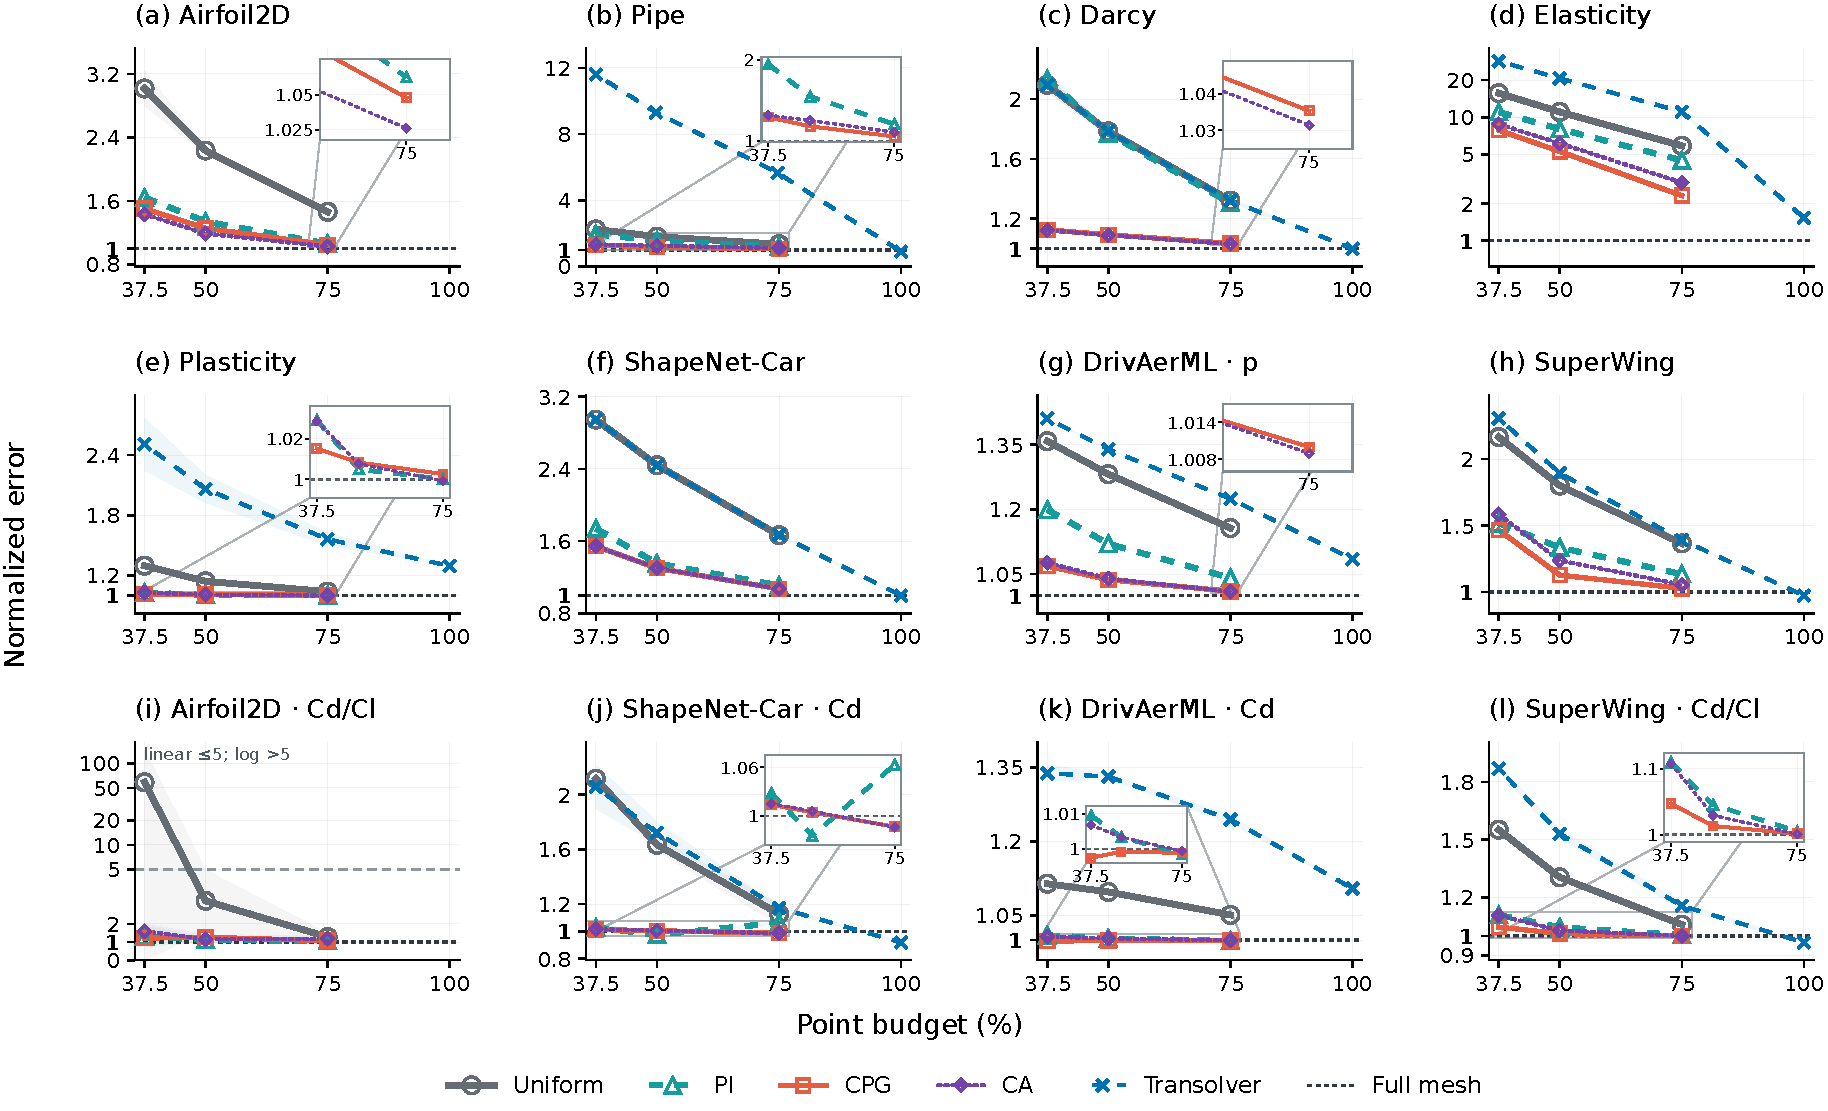
\includegraphics[width=\linewidth]{figures/appendix/budget_error_curves.pdf}
    \caption{\textbf{Error relative to the full mesh across point budgets.}
    Panels (a)--(h) show field metrics and (i)--(l) show aerodynamic quantities.
    Error definitions follow Section~\ref{sec:experiment_implementation}.
    Curves show means over three sampling seeds, with shaded bands indicating
    one sample standard deviation.
    The Airfoil $C_D/C_L$ metric is an absolute coefficient-ratio error before
    normalization, and panel (i) uses a logarithmic vertical axis. The dotted
    line at one marks full-mesh inference accuracy in every panel.}
    \label{fig:appendix_budget_curves}
\end{figure}

\clearpage
\subsection{Additional Field Visualization}
\label{app:field_visualizations}

The following pages connect the aggregate error profiles to spatial sampling
and reconstruction. Each page shows one held-out geometry at a $37.5\%$ point
budget with sampling seed zero. These examples were selected for visible
differences between sampling policies. Their annotations report errors for
the displayed case. The preceding curves summarize the test populations.

The first two rows show sampling locations and the policy's refinement
feature. Features are rescaled from each policy's minimum to its 99th
percentile for display, with larger values clipped at the upper end of the
colour scale. Uniform has no refinement feature. Each physical quantity then
has a ground-truth view and matched prediction and error rows. Field and
error ranges are shared across methods within that quantity. Colour-bar
arrows indicate values outside the displayed range. Component errors are
signed prediction-minus-ground-truth residuals. Magnitude rows show
nonnegative vector error norms, and Plasticity uses the temporal aggregation
specified below.

\subsubsection{Airfoil}
\label{app:vis_airfoil}

The pressure jump in this example makes errors in its location visible as
a narrow residual band. All three adaptive policies reduce the field error
relative to Uniform. PI gives the lowest error for this particular geometry,
illustrating the task-dependent policy ordering seen in the budget curves.

\begin{figure}[!ht]
    \centering
    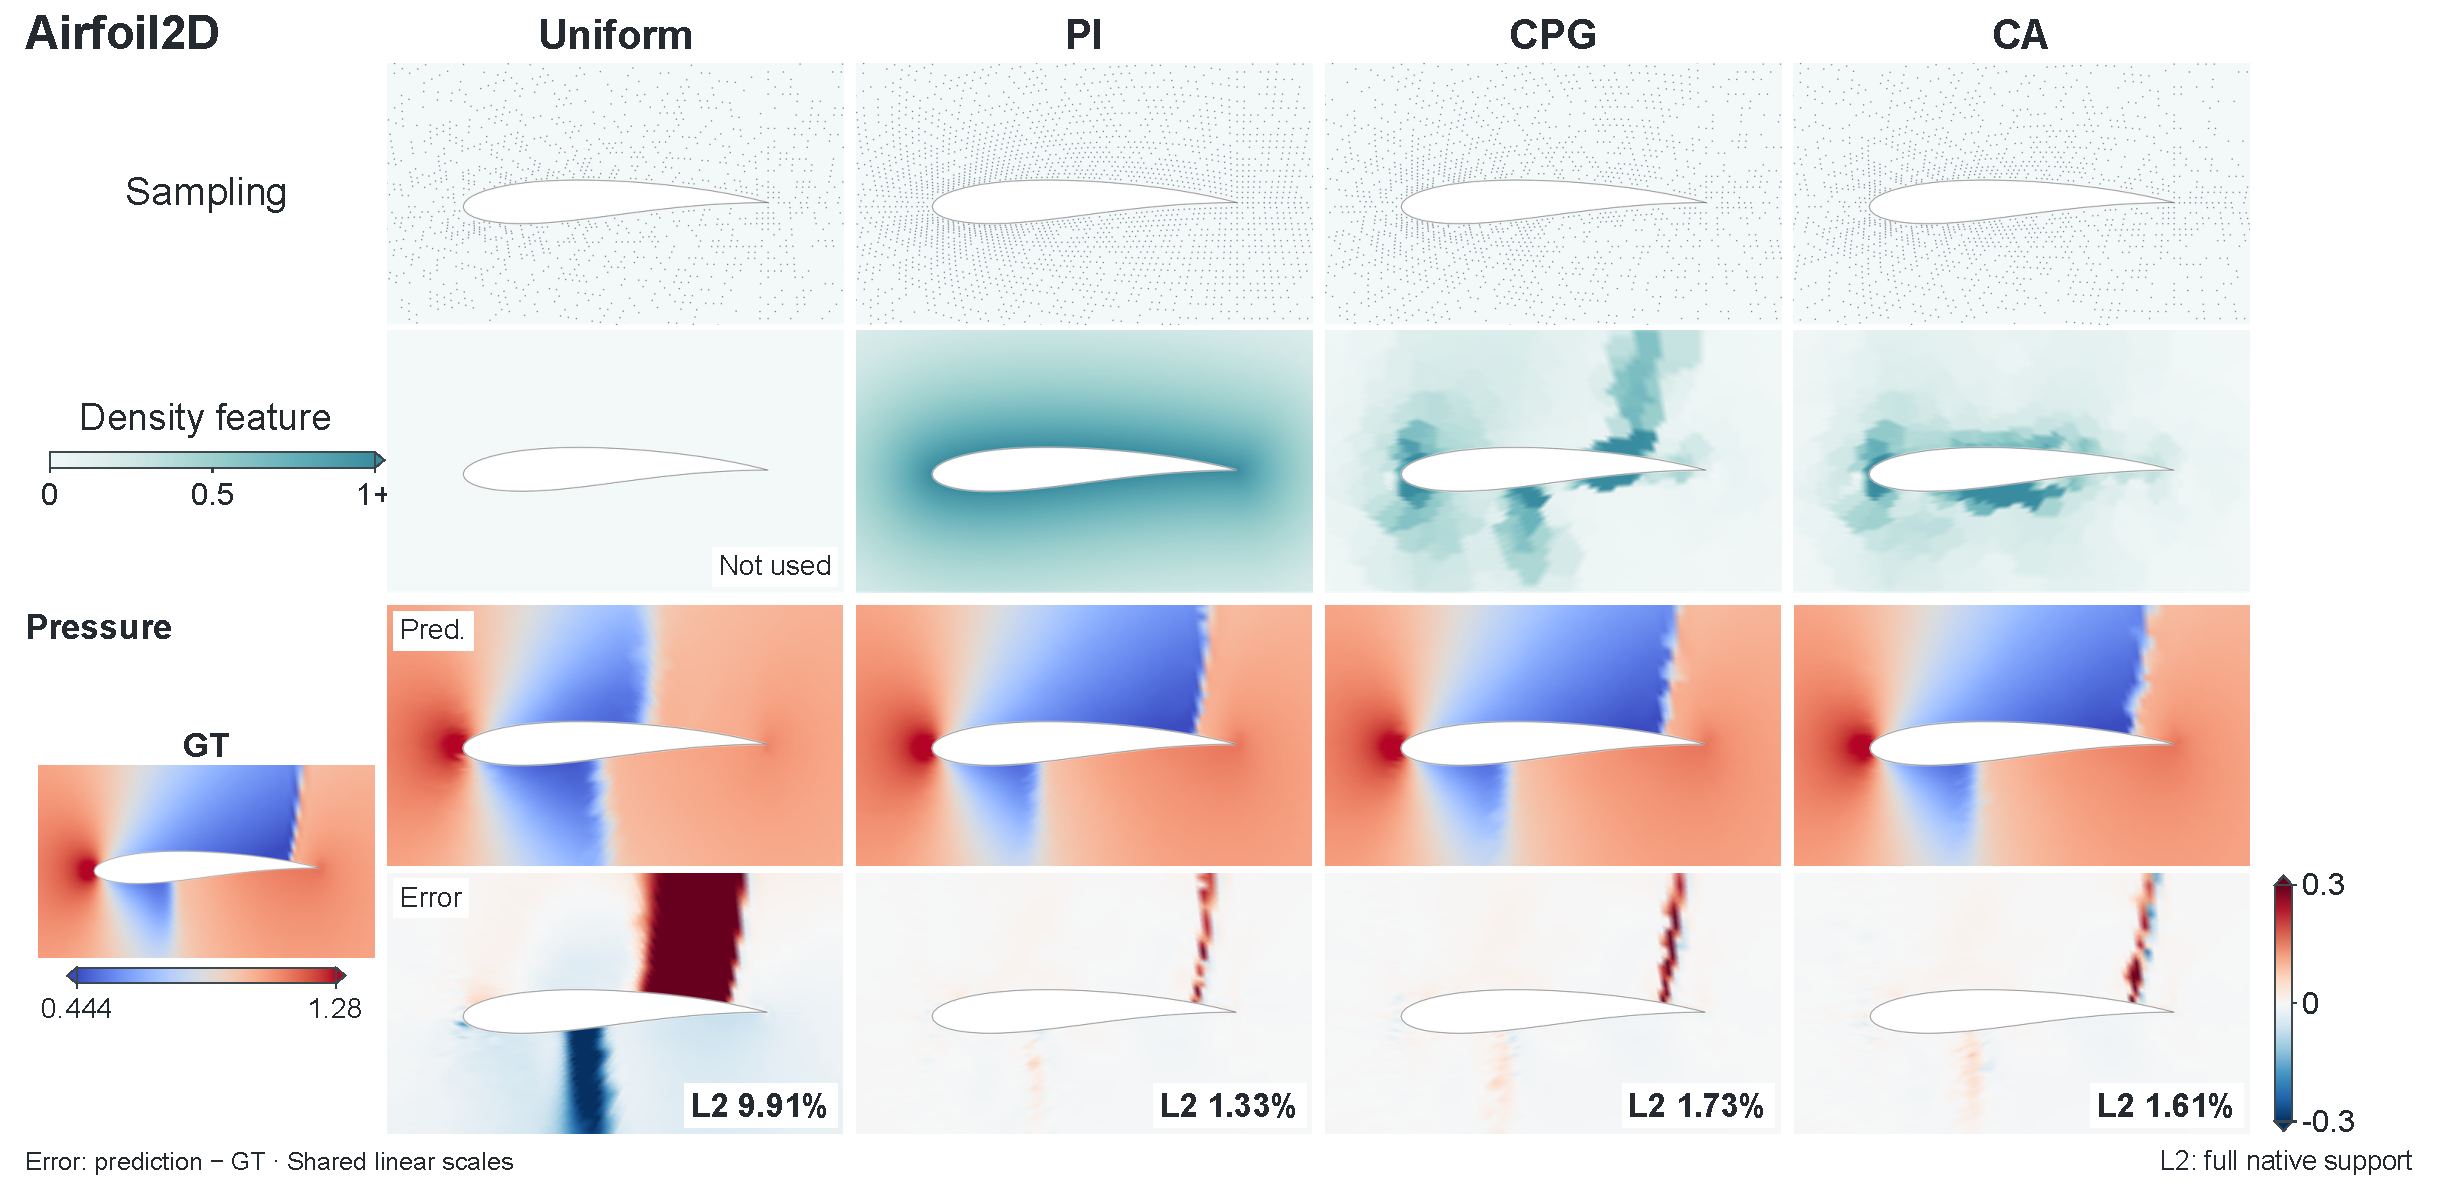
\includegraphics[width=\linewidth,height=.69\textheight,keepaspectratio]{figures/appendix/airfoil2d_fields.pdf}
    \caption{\textbf{Airfoil.} Sampling and pressure prediction.}
    \label{fig:appendix_airfoil}
\end{figure}

\clearpage
\subsubsection{Pipe}
\label{app:vis_pipe}

The predicted horizontal-velocity fields have similar overall structure,
while the shared residual scale exposes differences along the curved pipe.
CPG and CA reduce the error to $0.24\%$ and $0.30\%$, respectively,
compared with $1.31\%$ under Uniform sampling.

\begin{figure}[!ht]
    \centering
    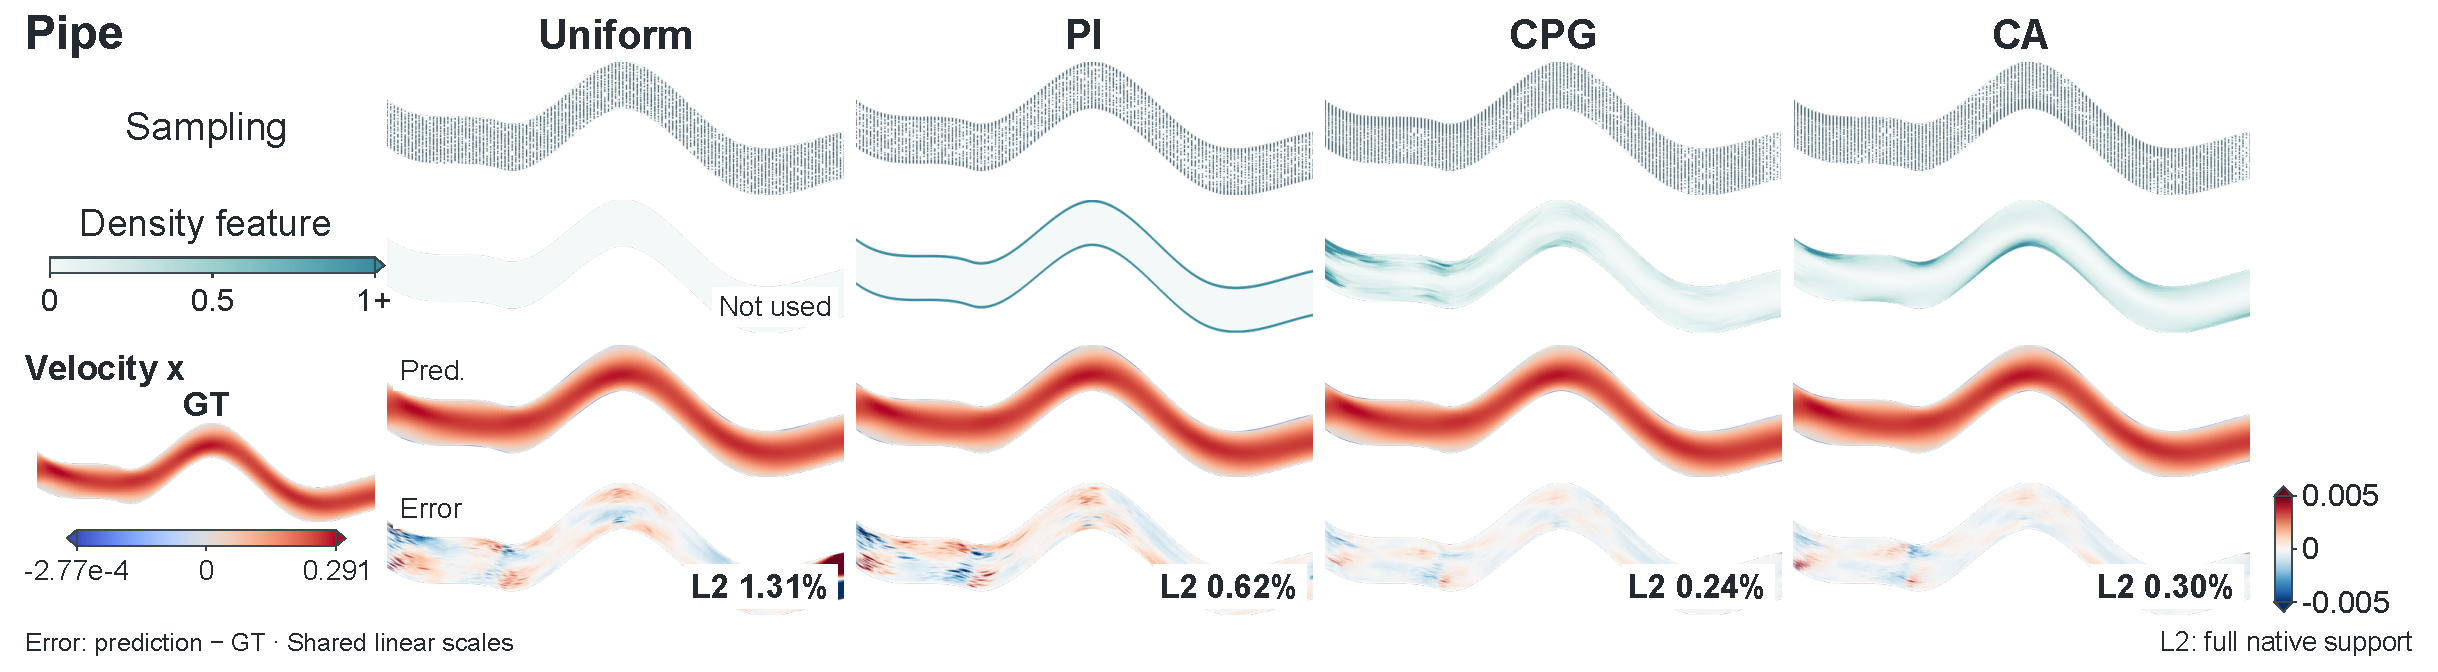
\includegraphics[width=\linewidth,height=.69\textheight,keepaspectratio]{figures/appendix/pipe_fields.pdf}
    \caption{\textbf{Pipe.} Sampling and horizontal velocity prediction.}
    \label{fig:appendix_pipe}
\end{figure}

\clearpage
\subsubsection{Darcy}
\label{app:vis_darcy}

The refinement policies assign different importance to regions of the
heterogeneous medium. The CPG and CA allocations produce similar solution
fields and smaller residuals than Uniform in this example, consistent with
their aggregate advantage on Darcy in Figure~\ref{fig:appendix_budget_curves}.

\begin{figure}[!ht]
    \centering
    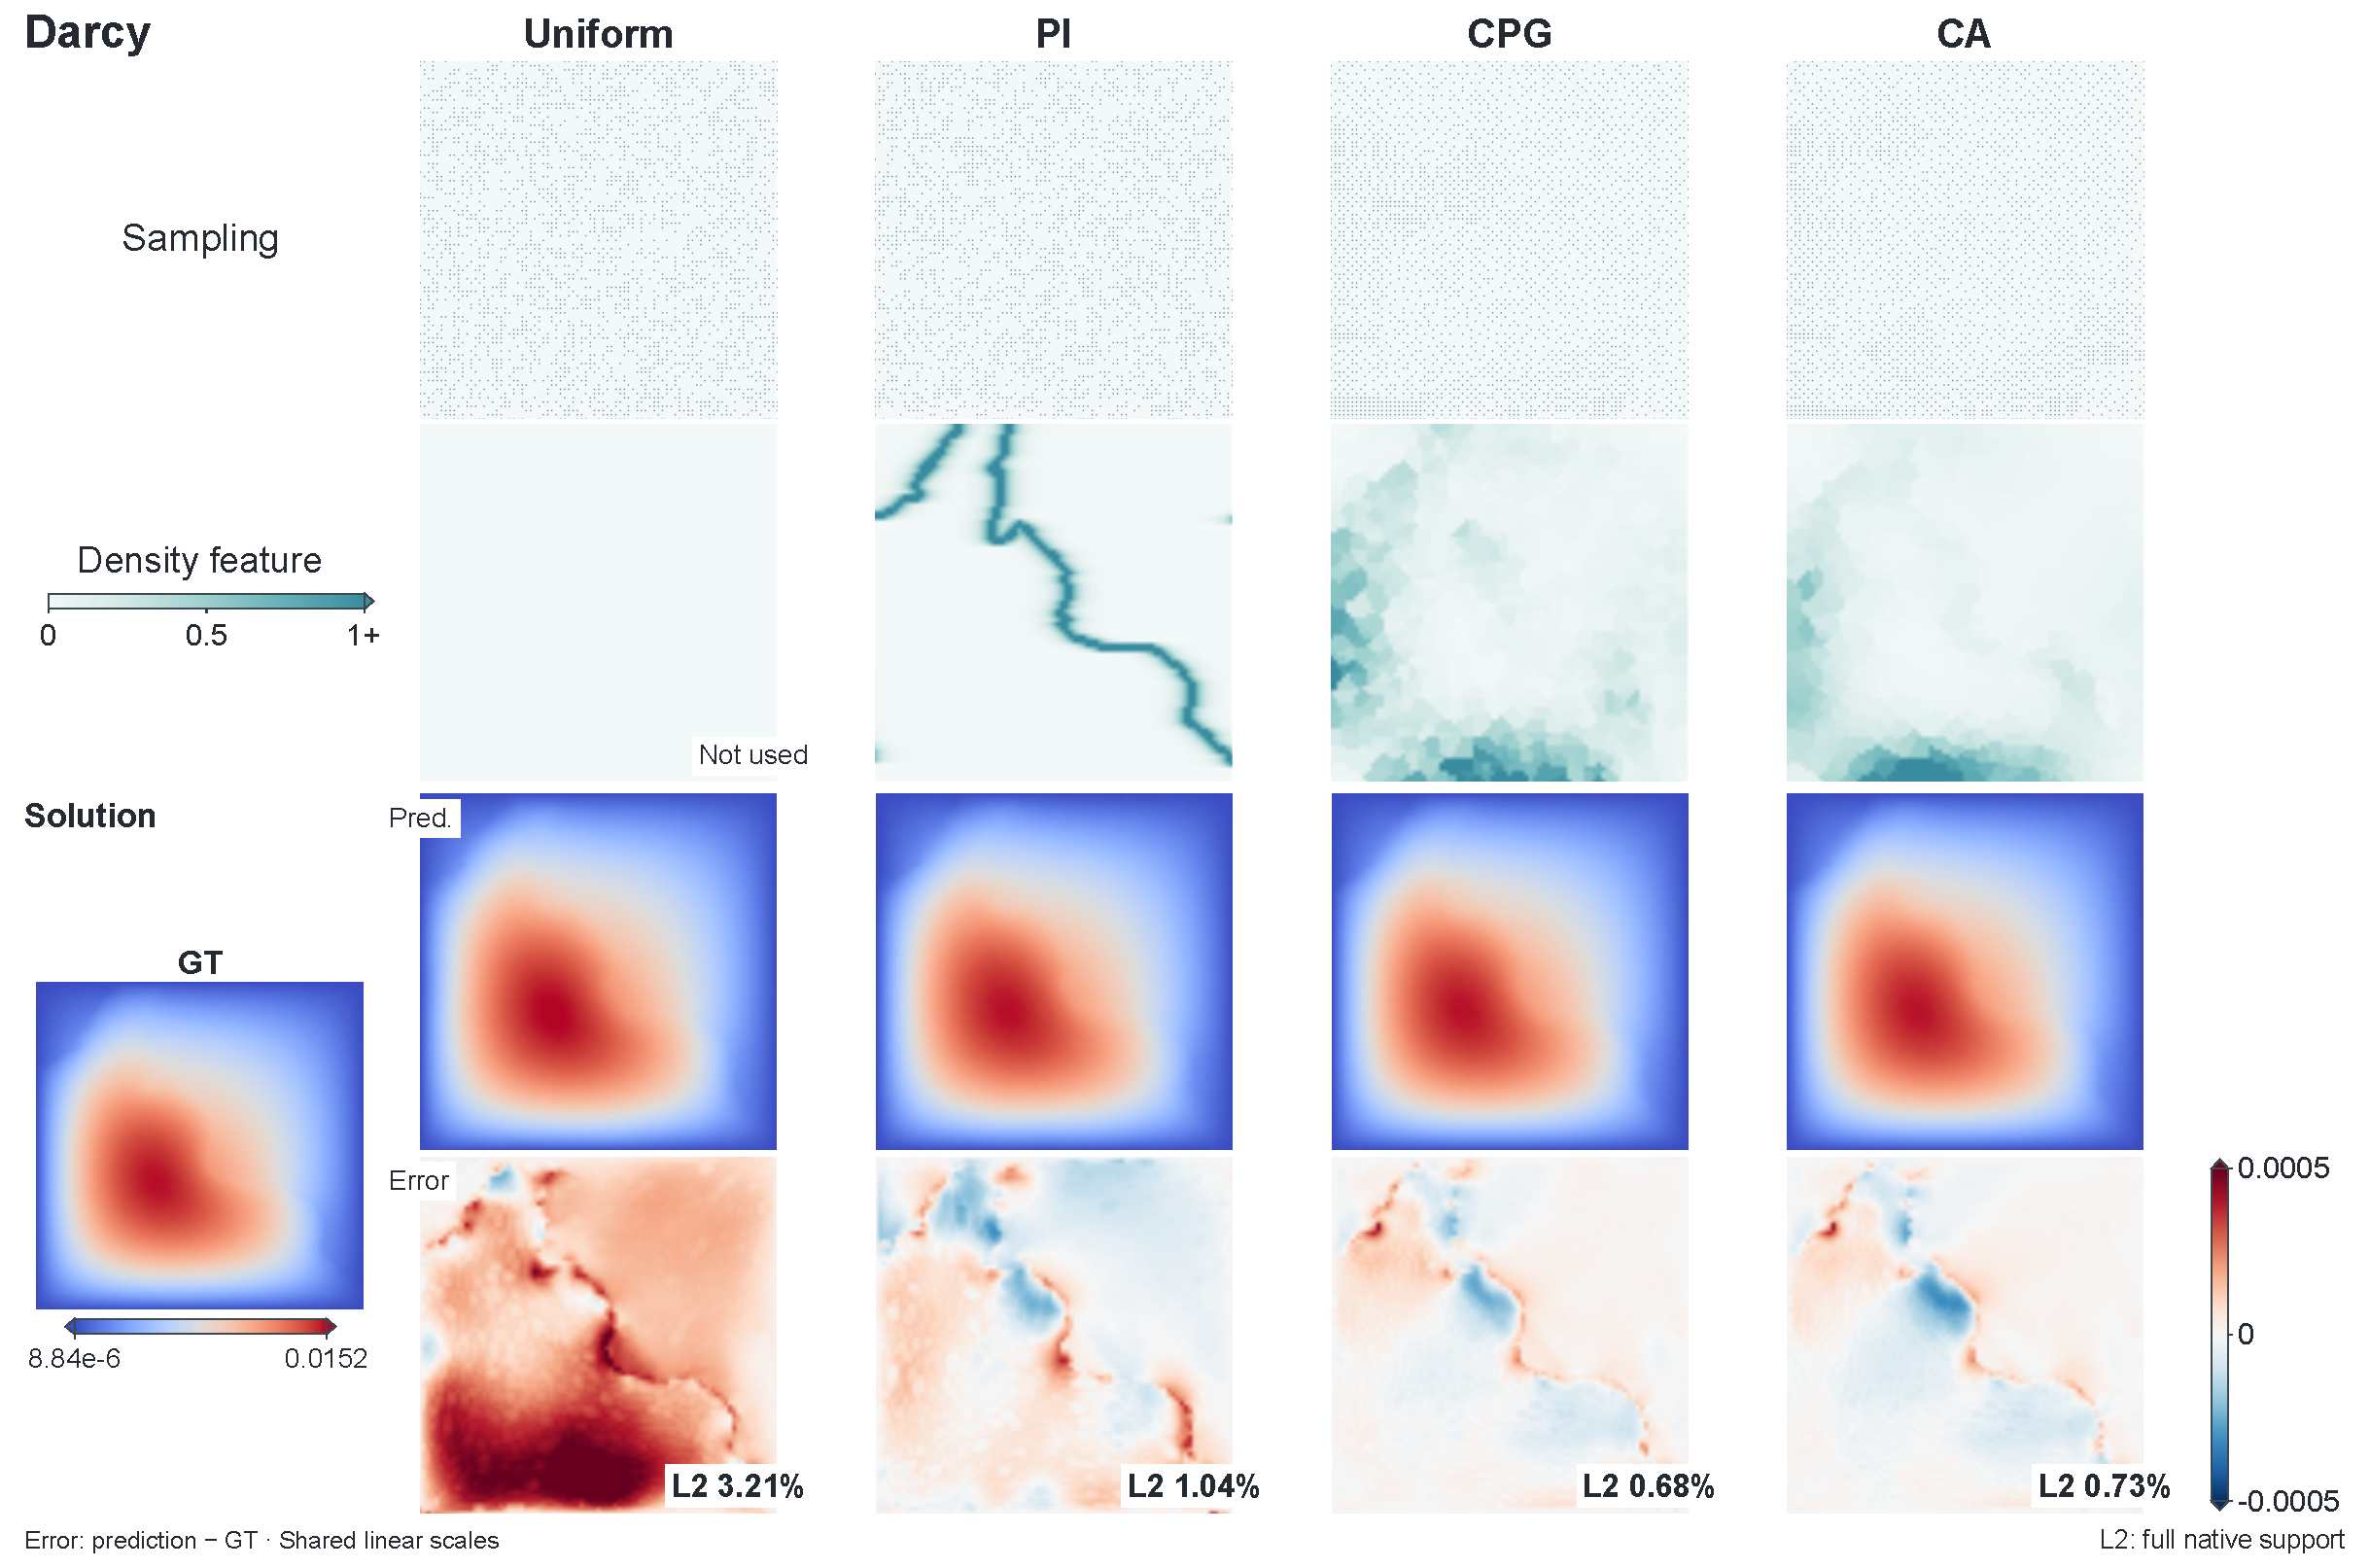
\includegraphics[width=\linewidth,height=.69\textheight,keepaspectratio]{figures/appendix/darcy_fields.pdf}
    \caption{\textbf{Darcy.} Sampling and pressure prediction.}
    \label{fig:appendix_darcy}
\end{figure}

\clearpage
\subsubsection{Elasticity}
\label{app:vis_elasticity}

The irregular hole creates localized stress structure. The residual views
show the reduction in reconstruction error around this region under adaptive
sampling. CPG and CA attain similar errors, with PI also improving
substantially upon the uniform allocation.

\begin{figure}[!ht]
    \centering
    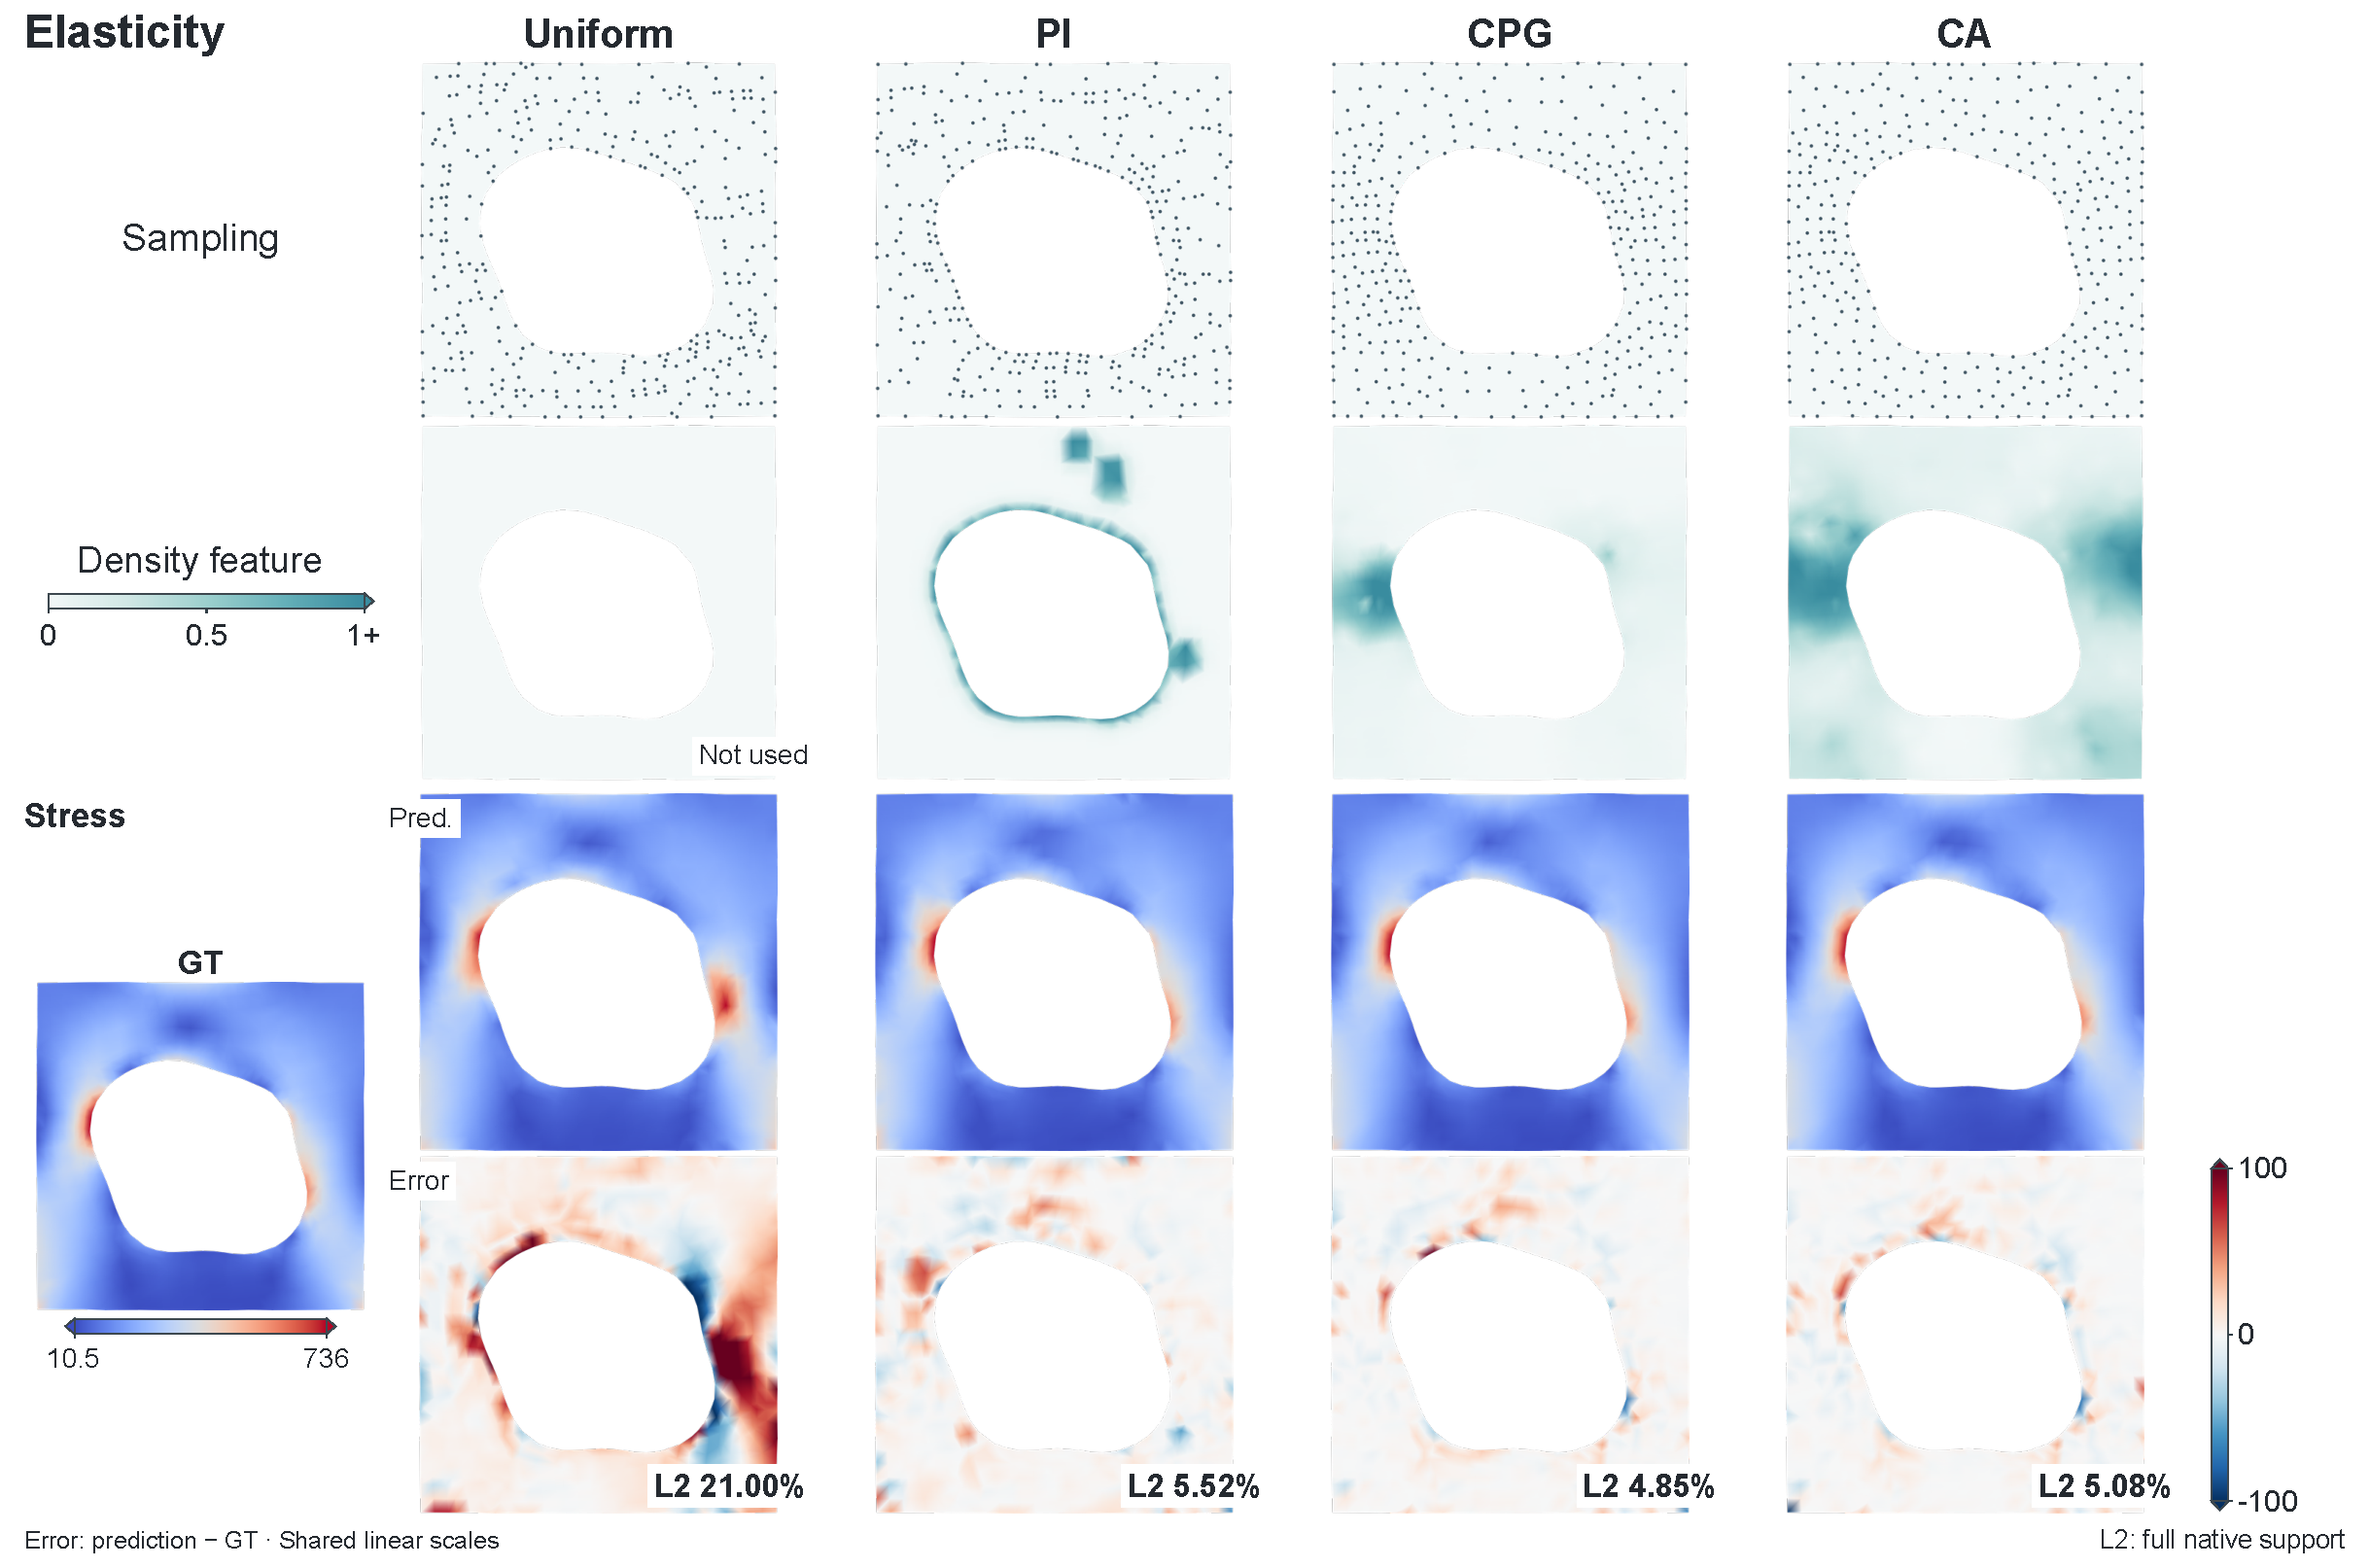
\includegraphics[width=\linewidth,height=.69\textheight,keepaspectratio]{figures/appendix/elasticity_fields.pdf}
    \caption{\textbf{Elasticity.} Sampling and stress prediction.}
    \label{fig:appendix_elasticity}
\end{figure}

\clearpage
\subsubsection{Plasticity}
\label{app:vis_plasticity}

Plasticity predicts a sequence of 20 displacement fields. We summarize all
recorded steps with equal weights, $w_t=1/20$, because the time grid is
uniform. The field rows show time-averaged components and displacement
magnitude. Component-error rows average the absolute residual at each step.
The magnitude-error row averages the vector residual norm. The annotated
$L_2$ errors use the weighted space--time fields over all 20 steps.

\begin{figure}[!ht]
    \centering
    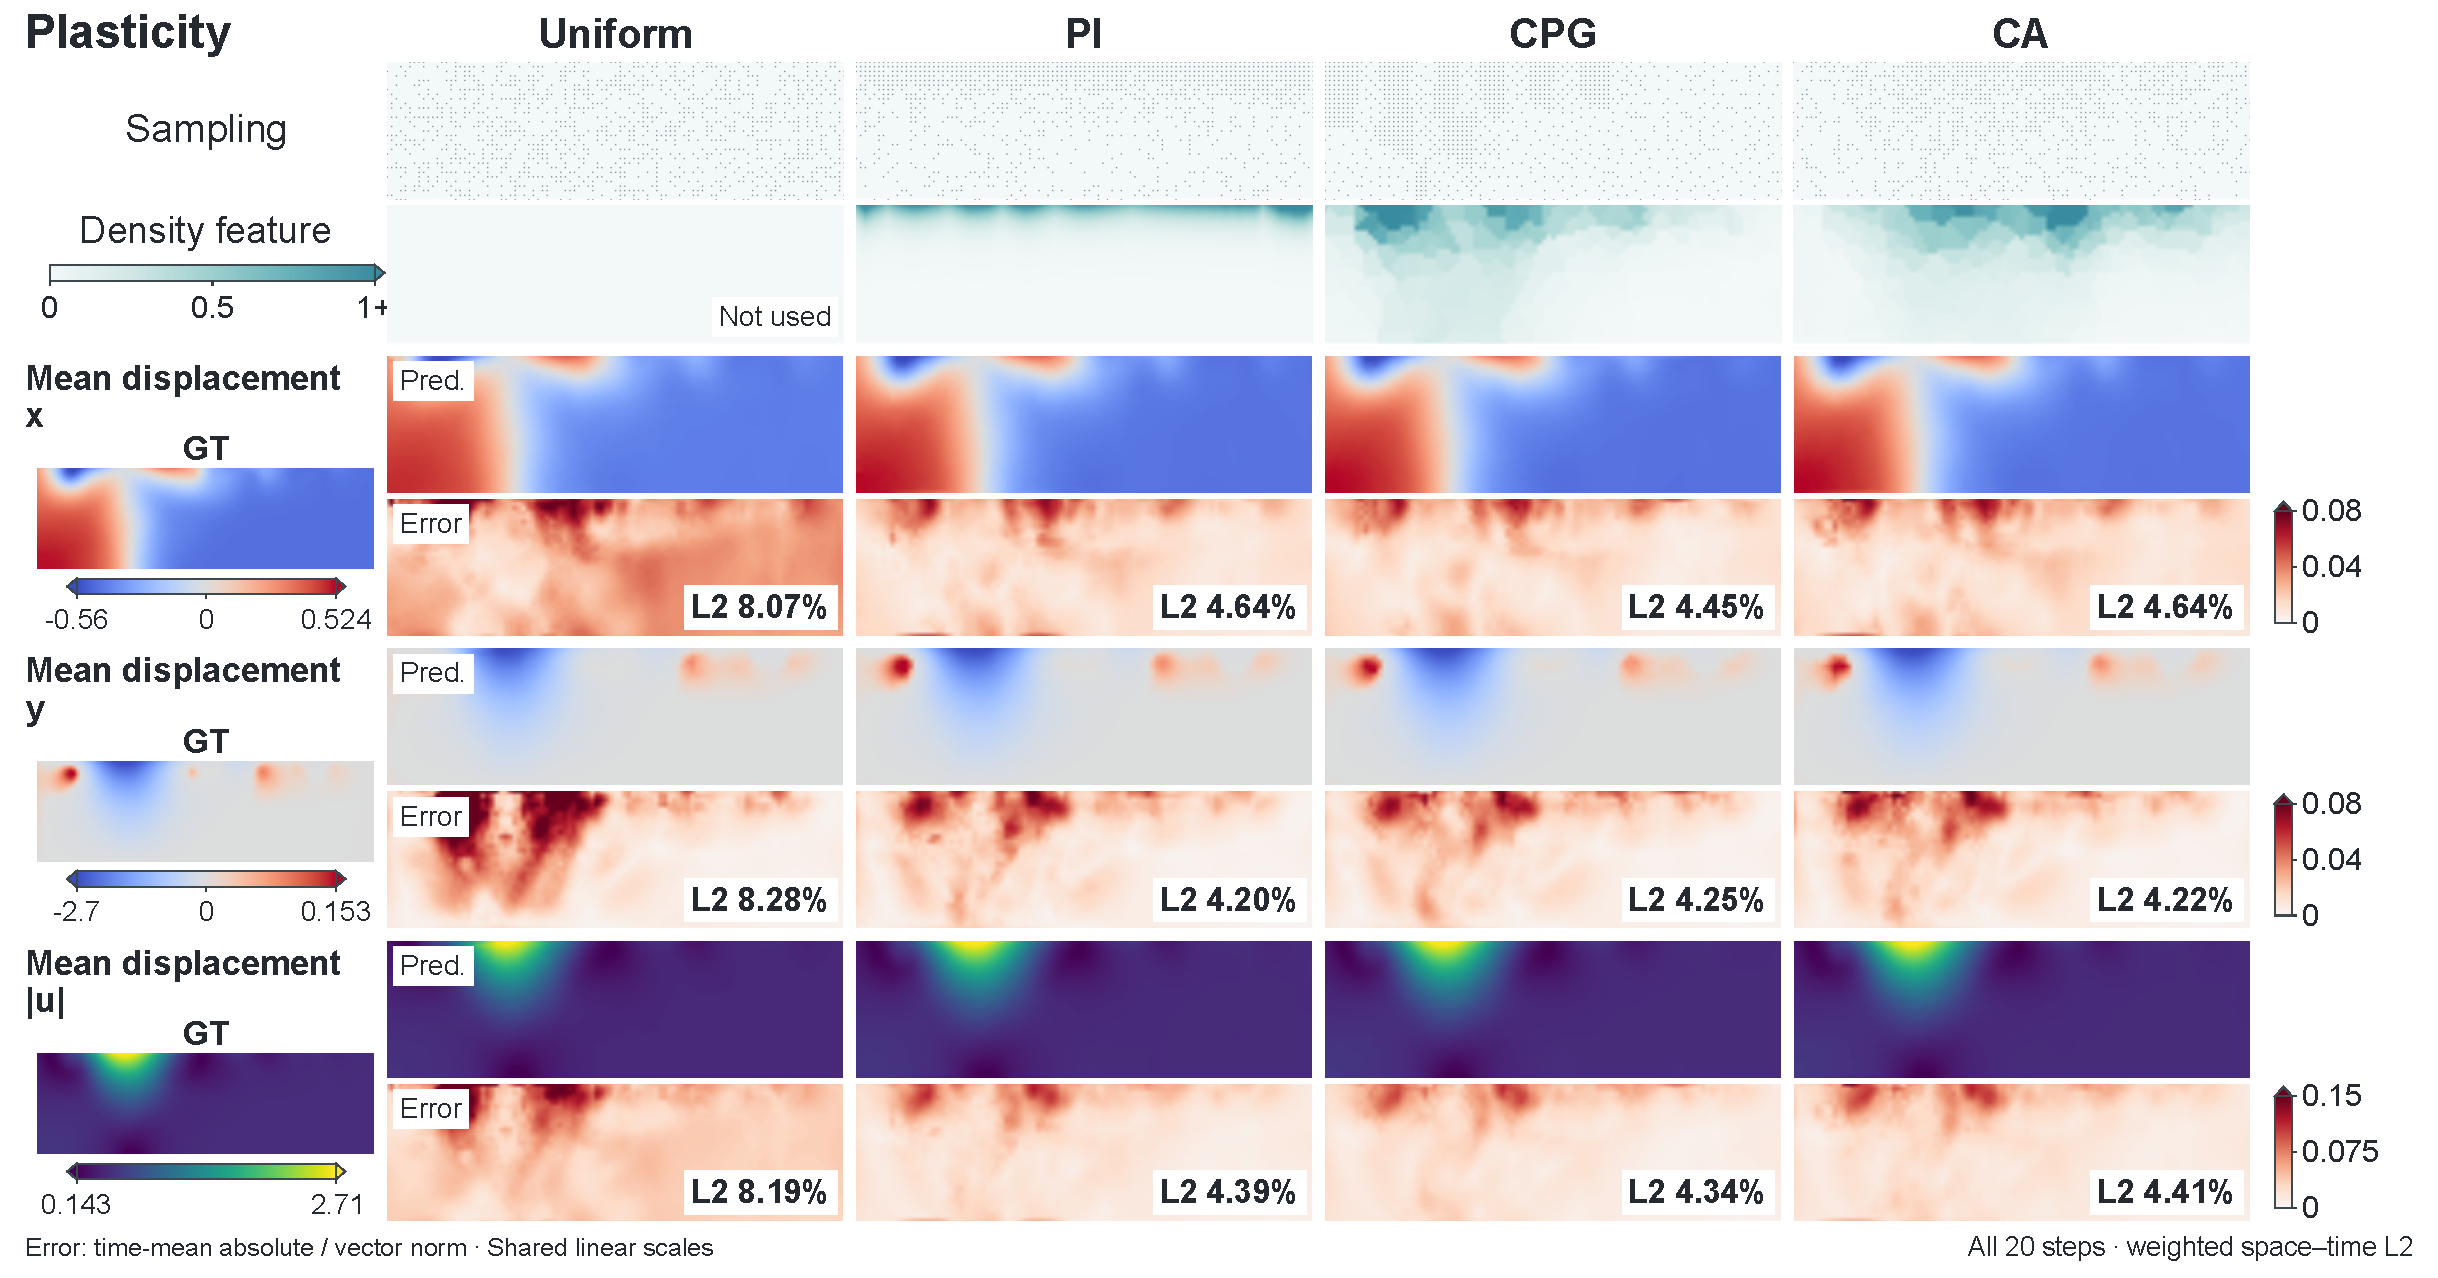
\includegraphics[width=\linewidth,height=.69\textheight,keepaspectratio]{figures/appendix/plasticity2d_fields.pdf}
    \caption{\textbf{Plasticity.} Sampling and displacement prediction.}
    \label{fig:appendix_plasticity}
\end{figure}

\clearpage
\subsubsection{ShapeNet-Car}
\label{app:vis_shapenet}

The automotive examples contain both surface and volumetric outputs.
For ShapeNet-Car, pressure is shown on the surface, and a fixed geometric
slice exposes the three velocity components and speed in the surrounding
volume. Error annotations use each field's full native support. This view
connects changes in point allocation to both pressure and velocity accuracy.

\begin{figure}[!ht]
    \centering
    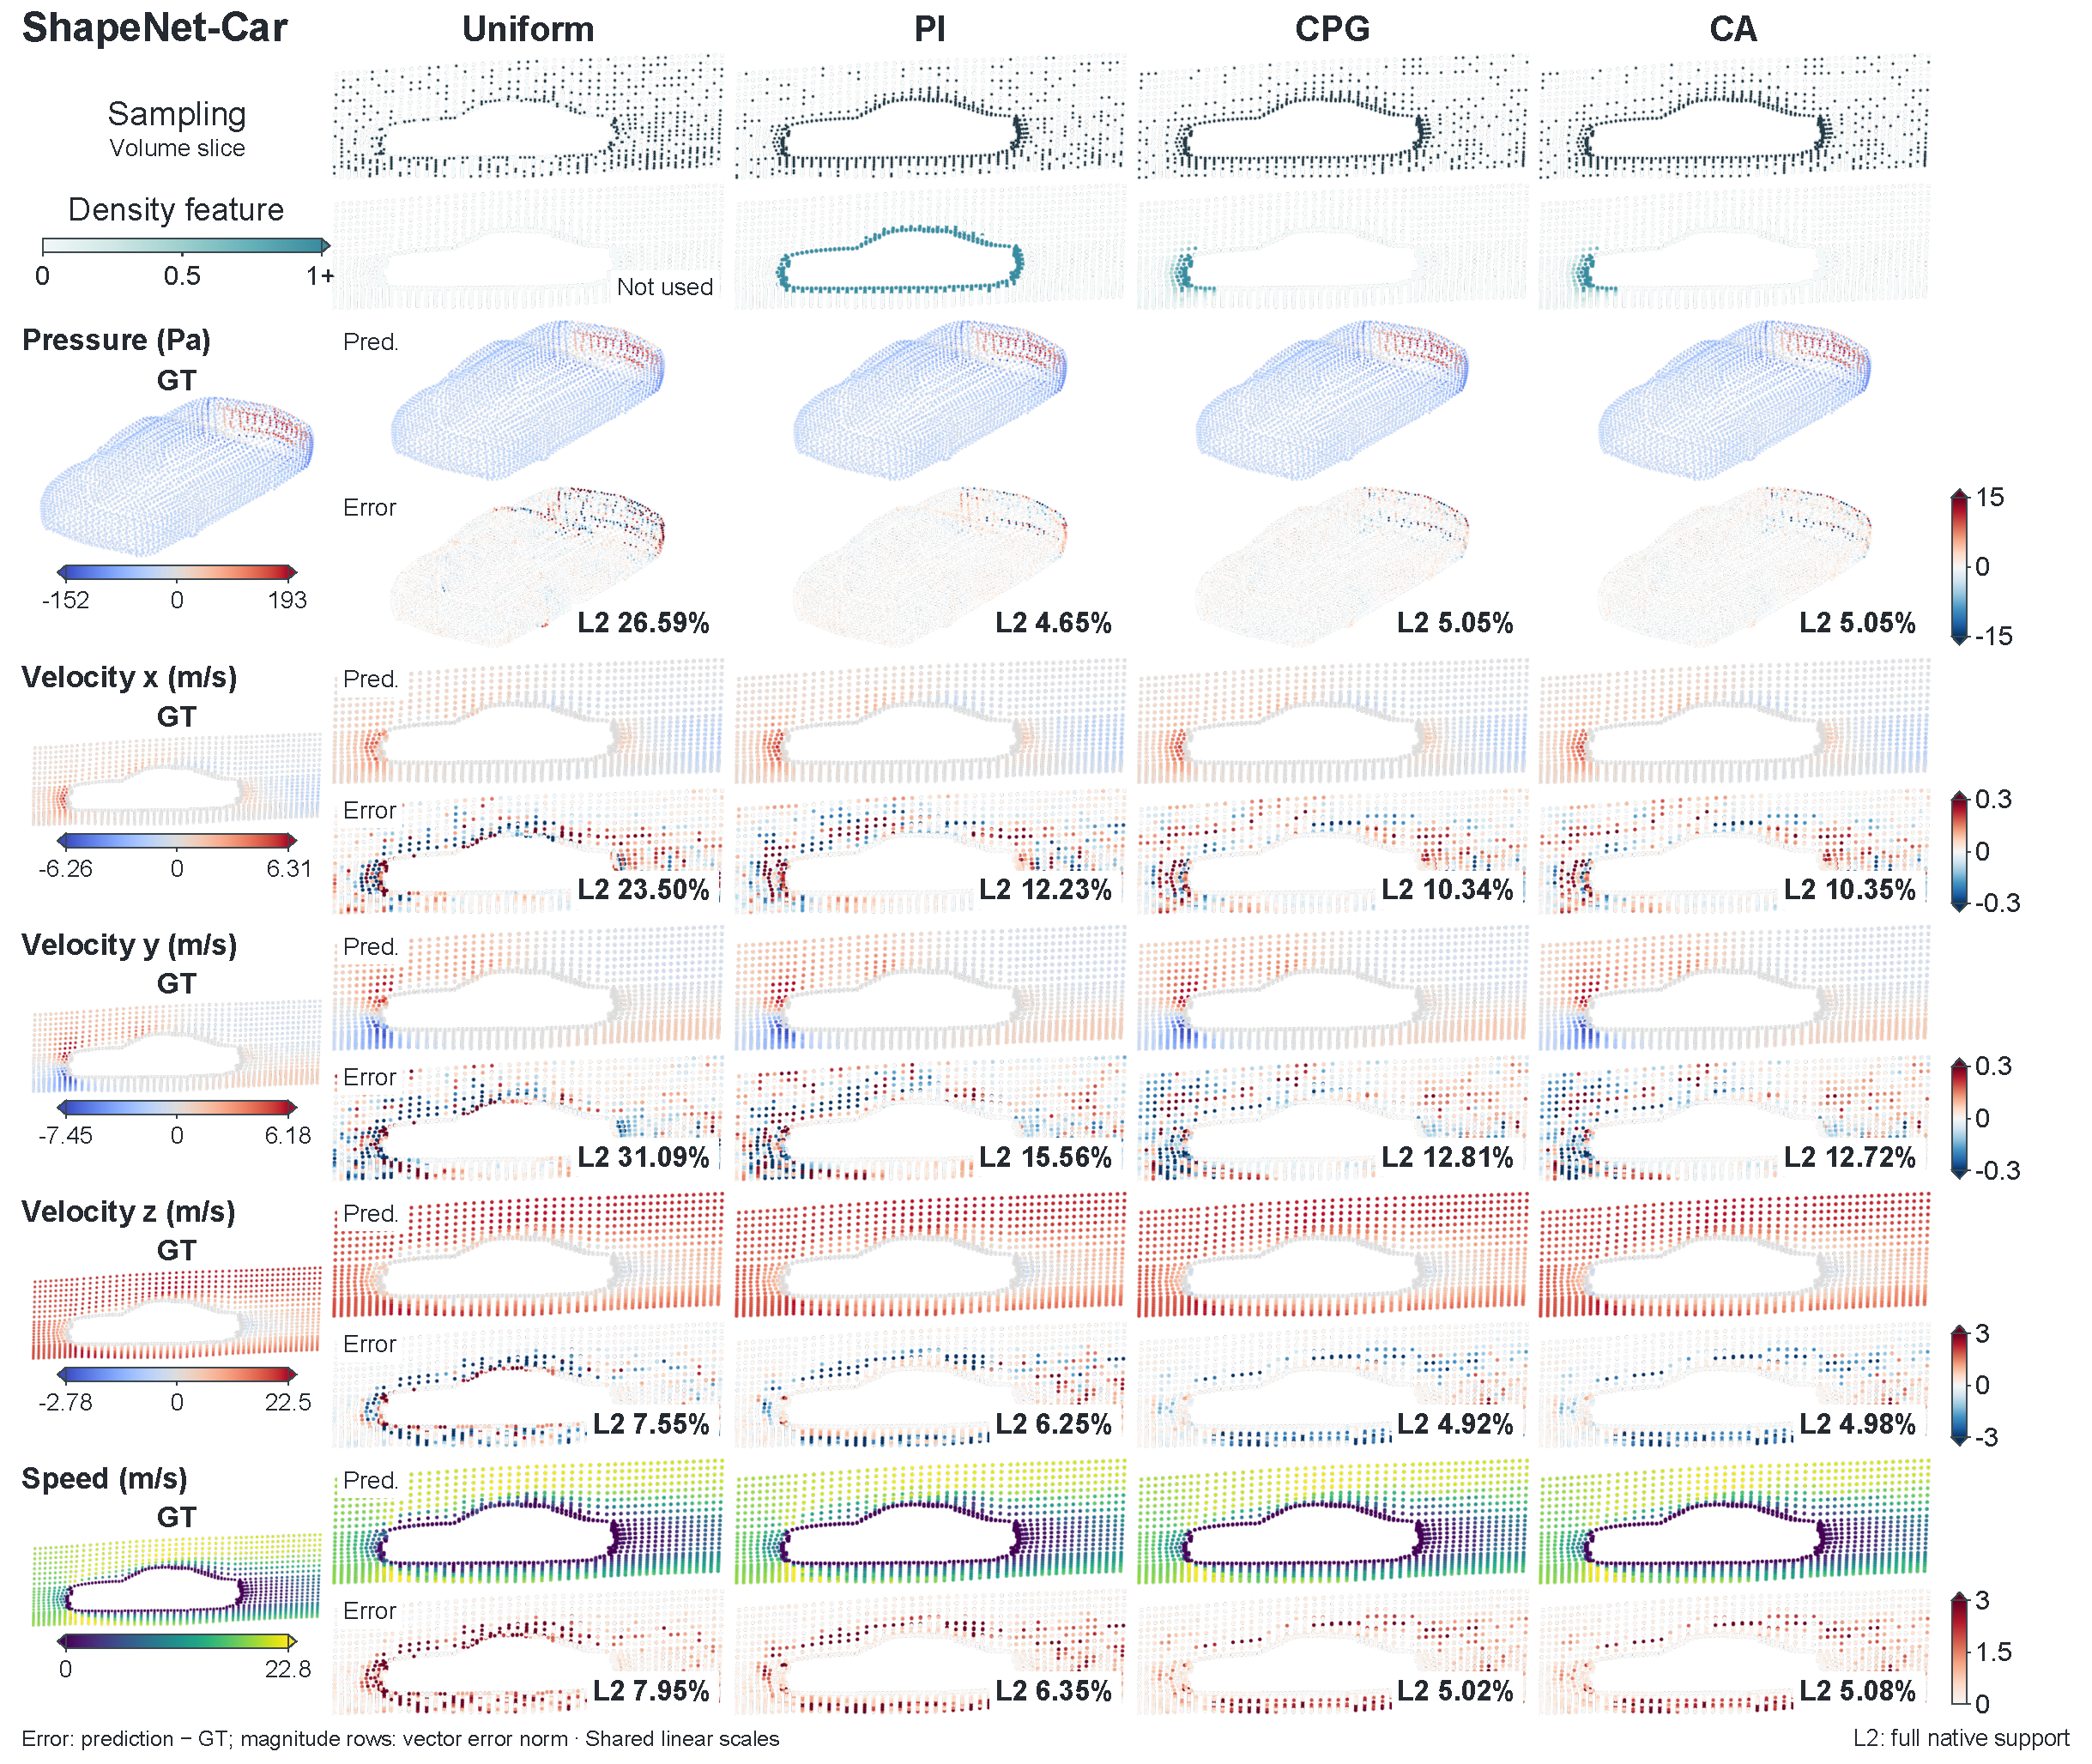
\includegraphics[width=\linewidth,height=.69\textheight,keepaspectratio]{figures/appendix/shapenet_car_fields.pdf}
    \caption{\textbf{ShapeNet-Car.} Sampling and prediction of surface pressure
    and volumetric velocity.}
    \label{fig:appendix_shapenet}
\end{figure}

\clearpage
\subsubsection{DrivAerML}
\label{app:vis_drivaer}

DrivAerML provides pressure and wall-shear-stress predictions on the same
vehicle surface. We reuse each pressure sampler's point indices for the
frozen wall-shear-stress operator. The figure therefore shows how these
allocations affect pressure, all three shear components, and their vector
magnitude on a shared geometry.

\begin{figure}[!ht]
    \centering
    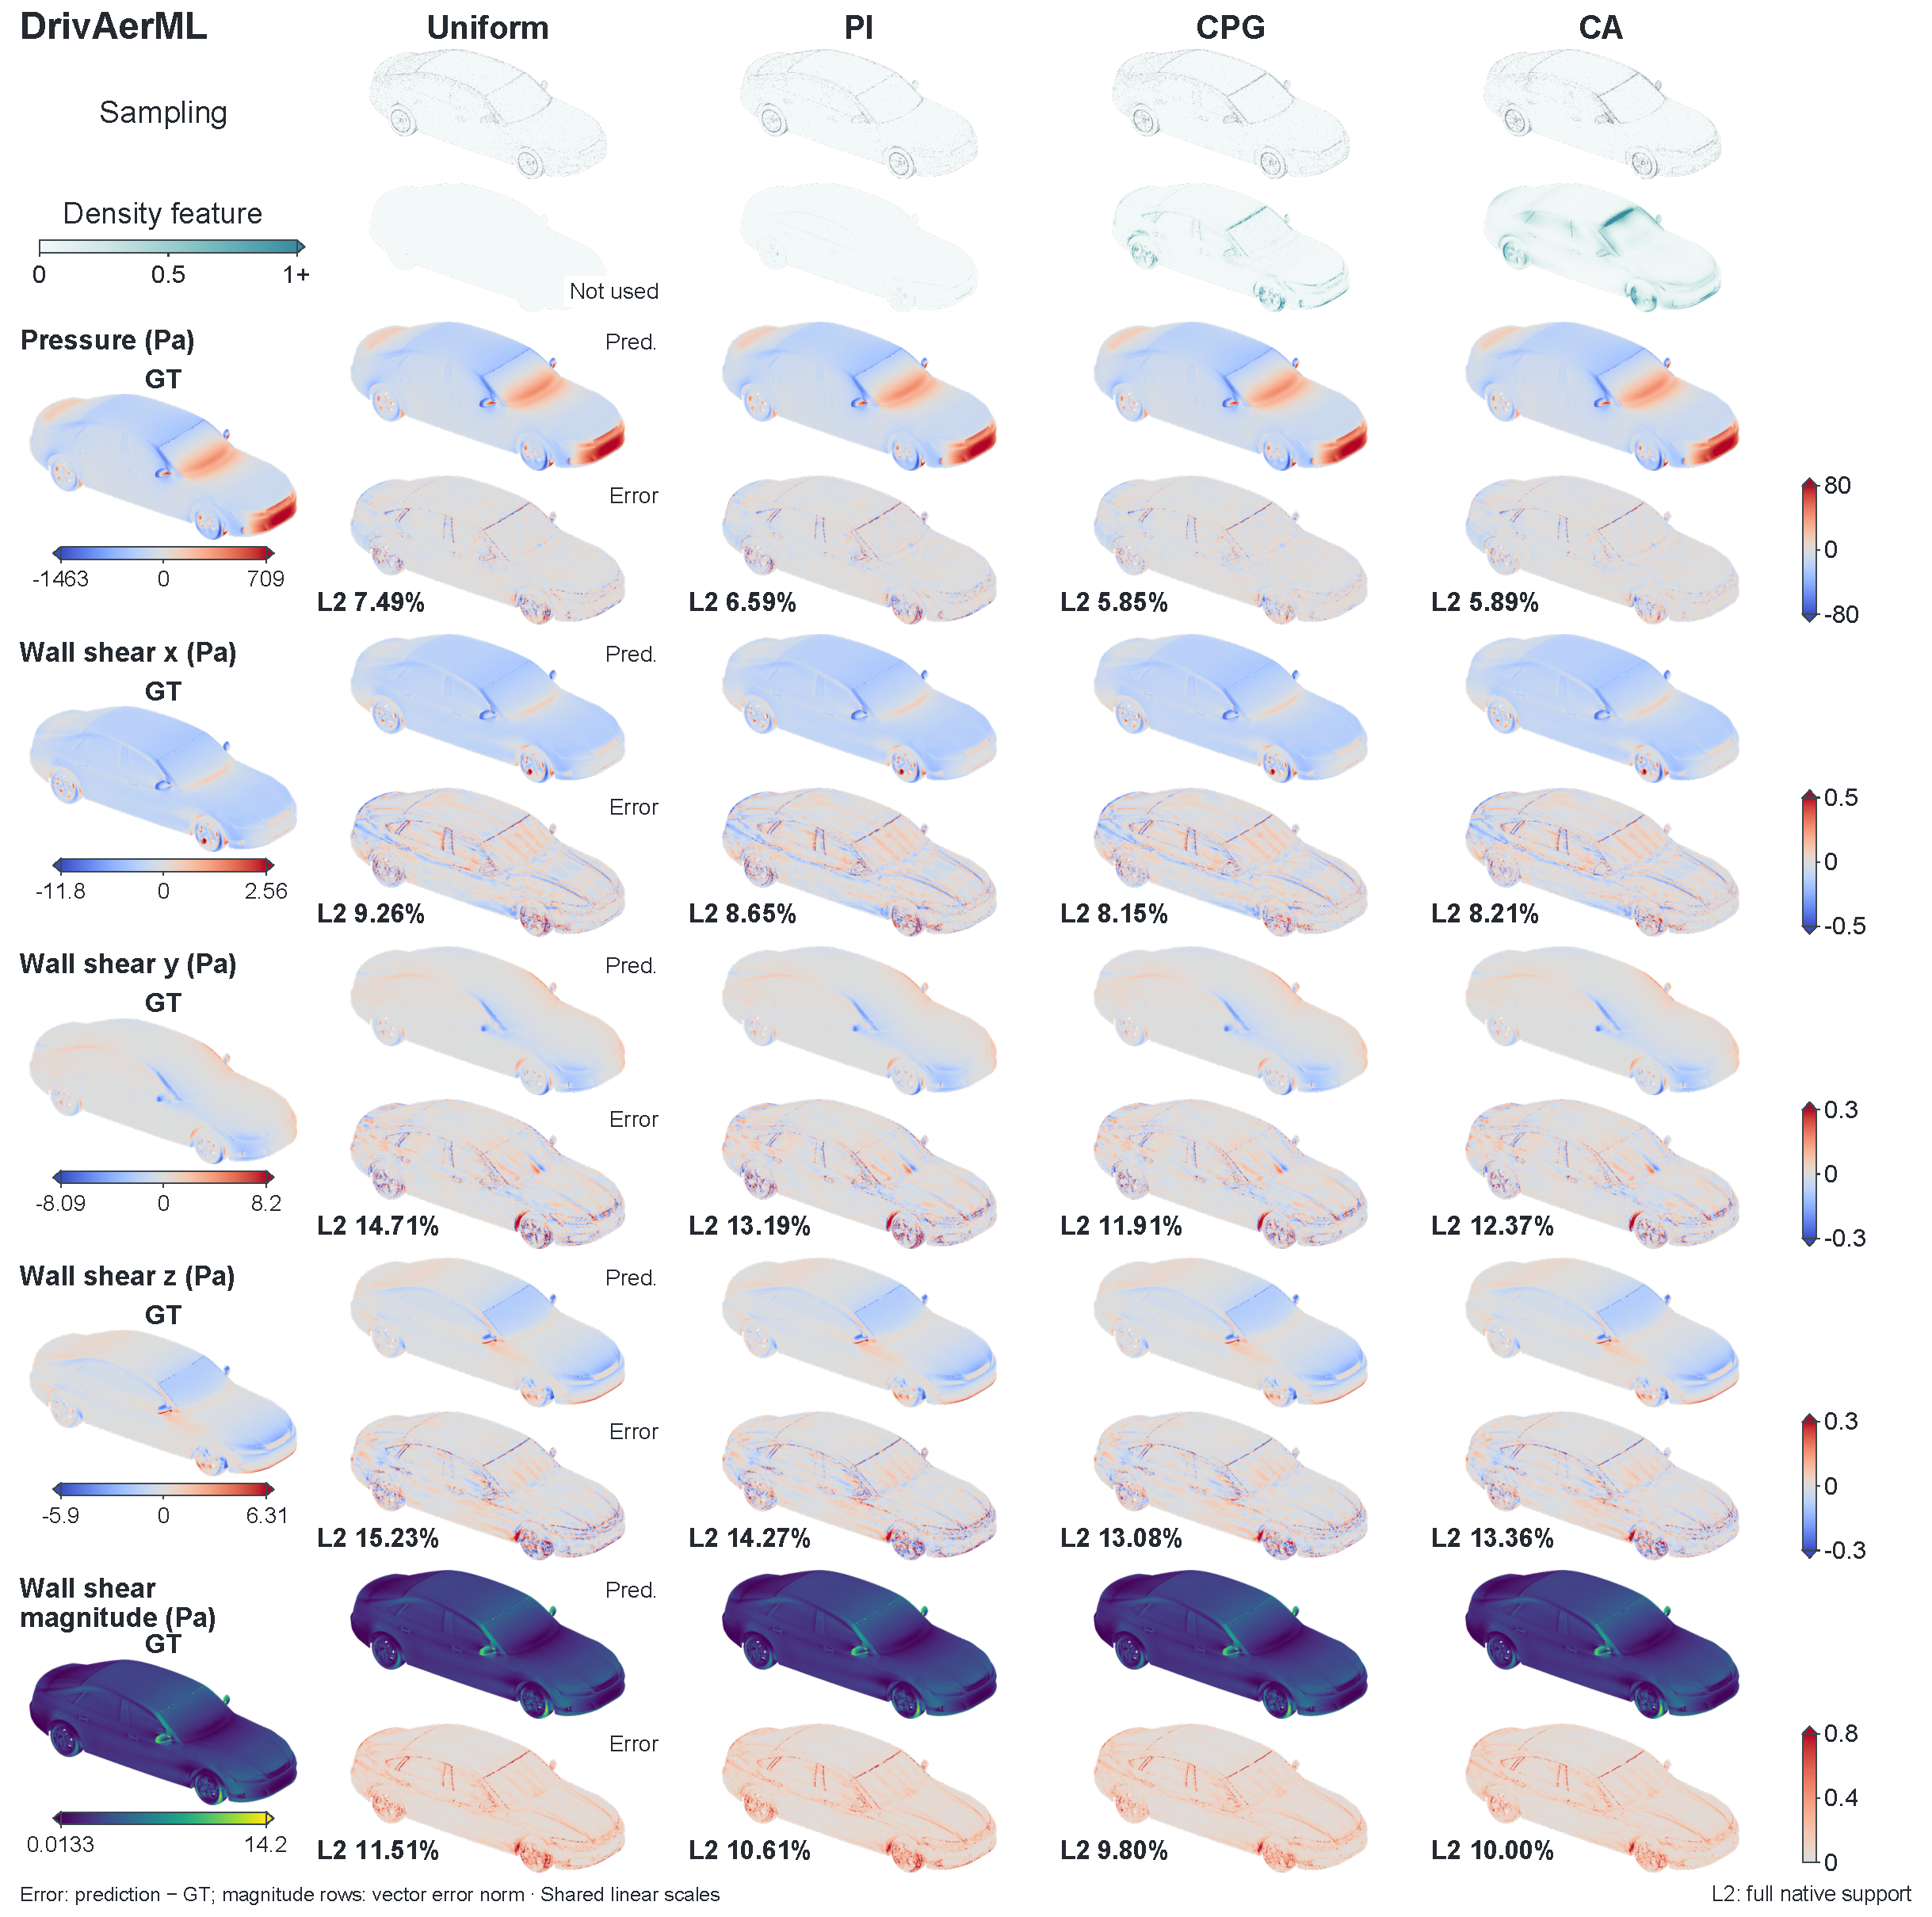
\includegraphics[width=\linewidth,height=.69\textheight,keepaspectratio]{figures/appendix/driverml_fields.pdf}
    \caption{\textbf{DrivAerML.} Sampling and prediction of surface pressure
    and wall shear stress.}
    \label{fig:appendix_drivaer}
\end{figure}

\clearpage
\subsubsection{SuperWing}
\label{app:vis_superwing}

The SuperWing page retains pressure and both friction components, together
with friction magnitude. The stored friction-channel scaling factors are
undone before visualization. Policy ordering varies across these outputs:
CPG gives the smallest pressure error for this wing, while PI gives the
smallest tangent-friction error. The individual rows expose this variation
beyond the joint field metric.

\begin{figure}[!ht]
    \centering
    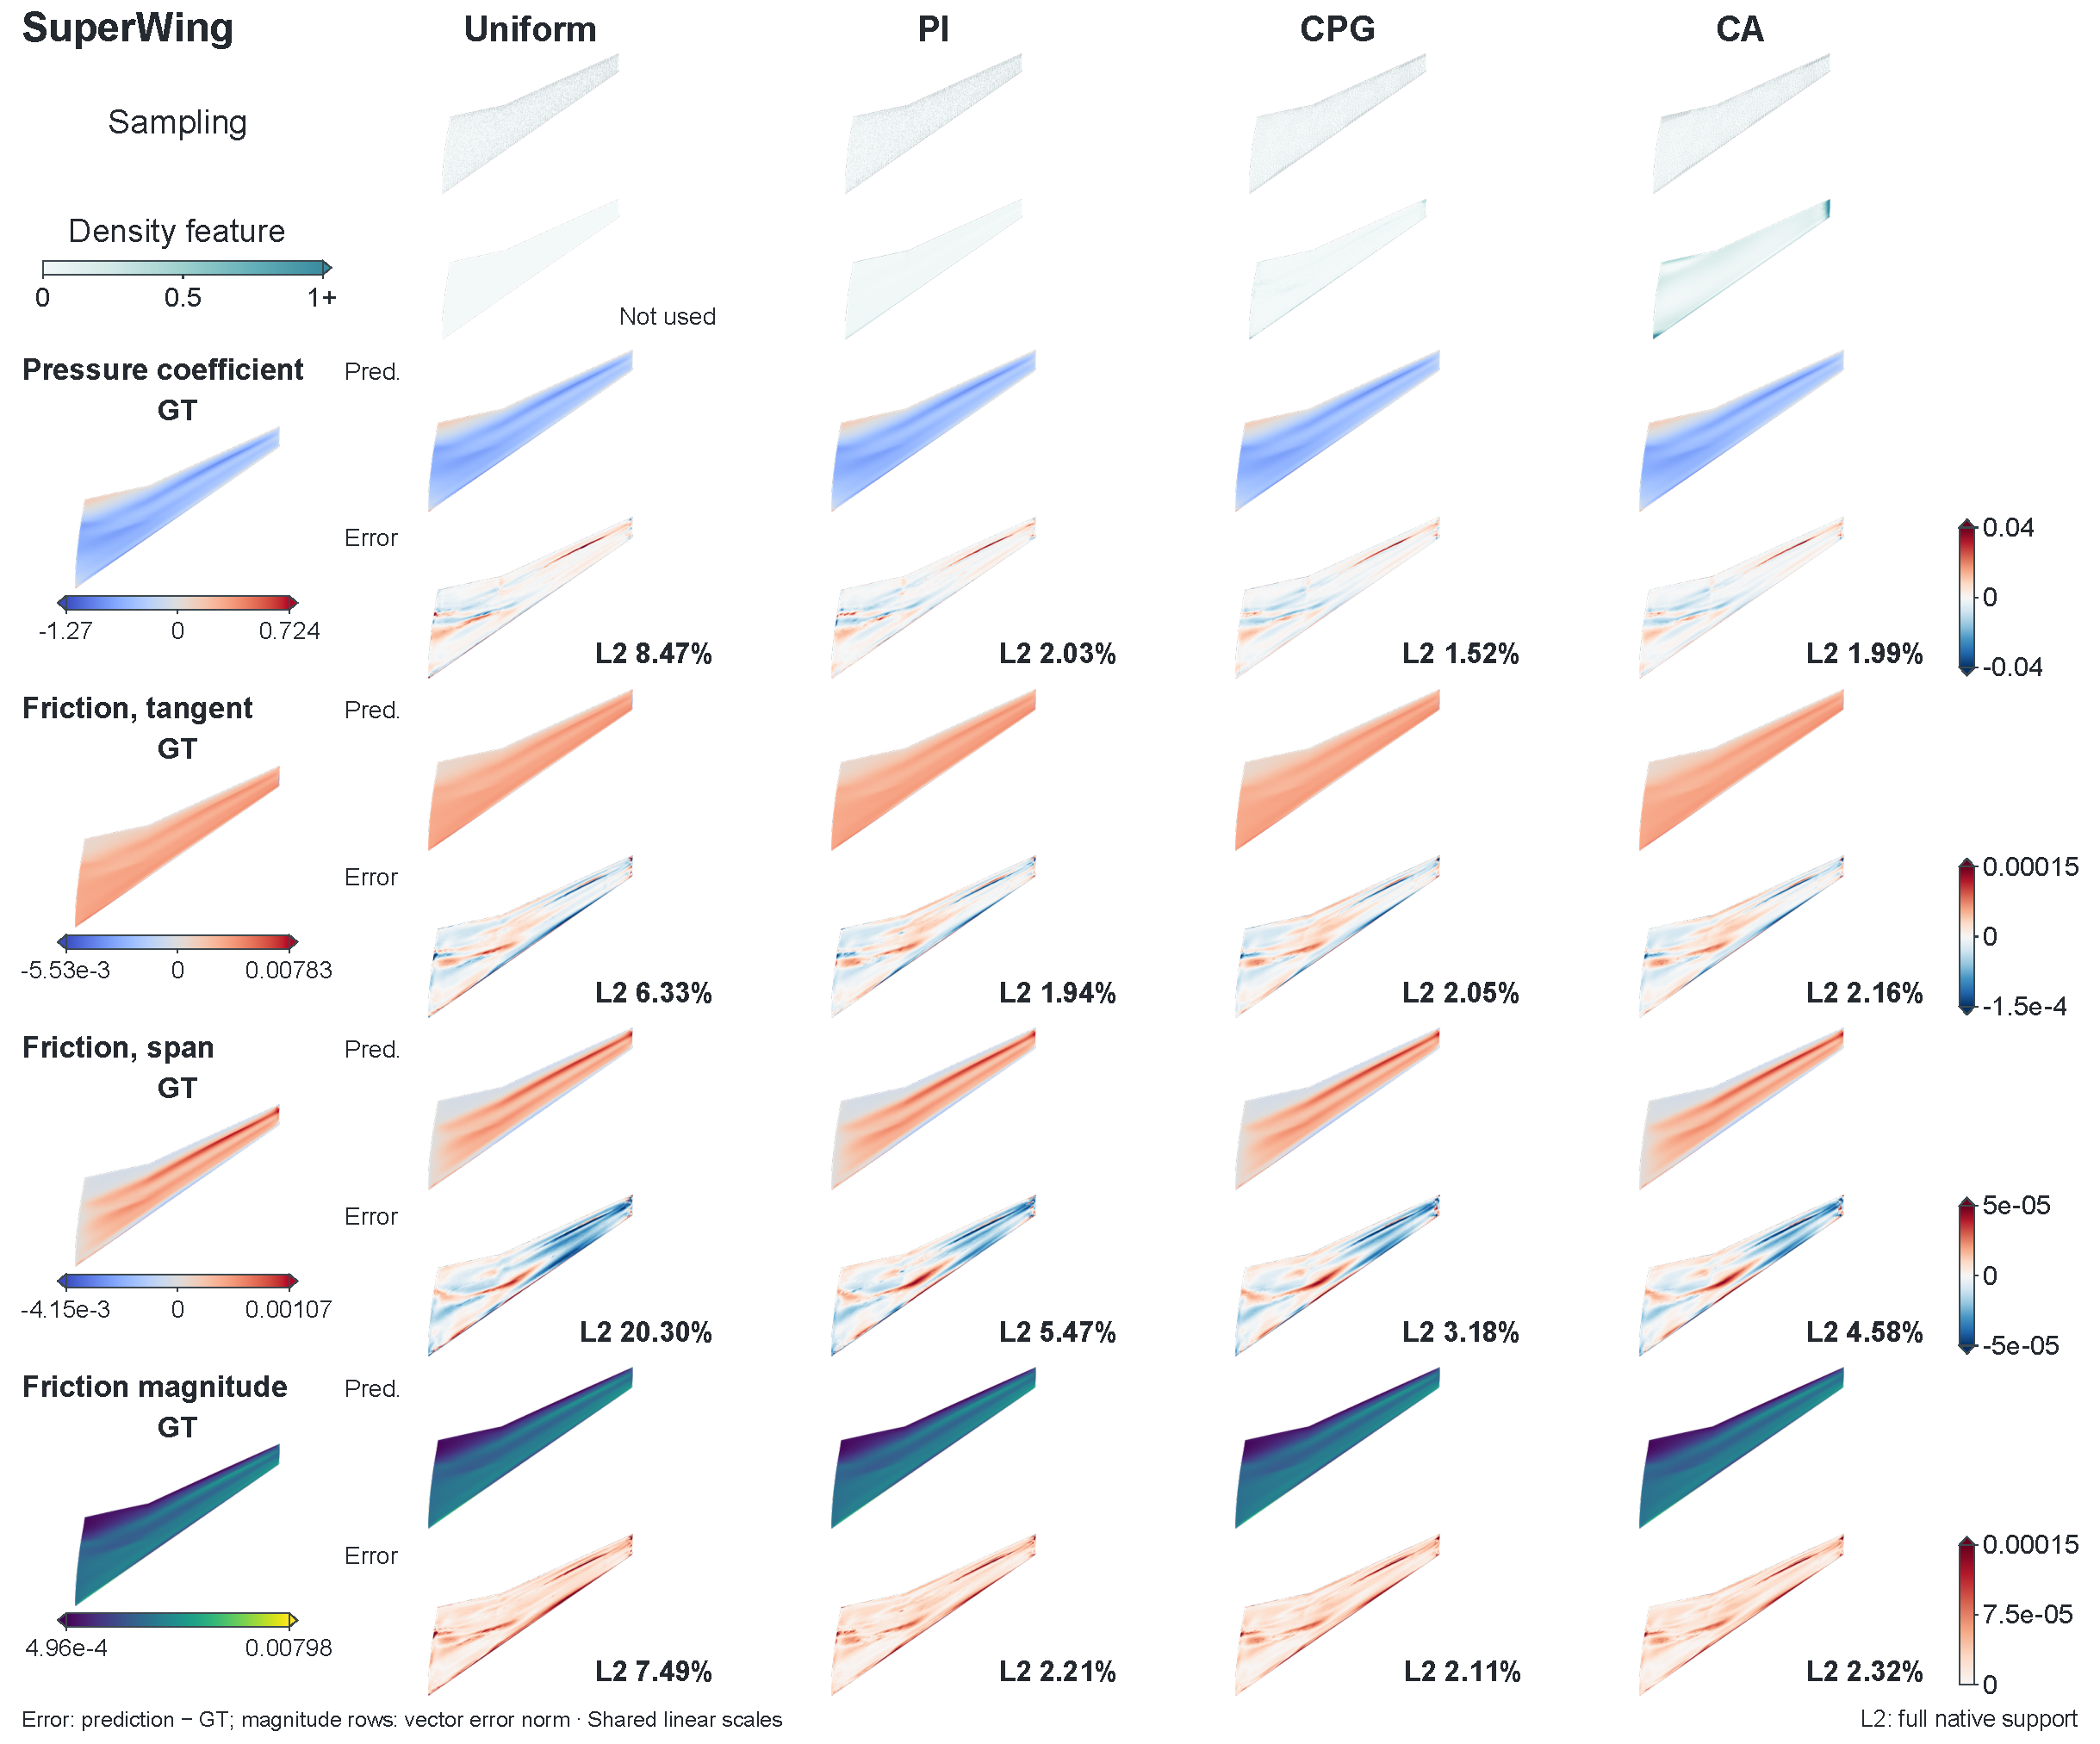
\includegraphics[width=\linewidth,height=.69\textheight,keepaspectratio]{figures/appendix/superwing_fields.pdf}
    \caption{\textbf{SuperWing.} Sampling and prediction of pressure
    and skin-friction coefficients.}
    \label{fig:appendix_superwing}
\end{figure}

\FloatBarrier
\section*{Acknowledgements}

We used large language models to assist with literature discovery and to edit and polish the manuscript.
The authors checked the cited literature against the original sources and reviewed and revised the
AI-assisted edits. All final research and editorial decisions were made by the authors, who take full
responsibility for the content, accuracy, originality, and integrity of this work.
\end{document}
